\documentclass[conference]{IEEEtran}
\IEEEoverridecommandlockouts
% The preceding line is only needed to identify funding in the first footnote. If that is unneeded, please comment it out.
\usepackage{cite}
\usepackage{amsmath,amssymb,amsfonts}
\usepackage{algorithmic}
\usepackage{algorithm}
\usepackage{graphicx}
\usepackage{textcomp}
\usepackage{comment}
\def\BibTeX{{\rm B\kern-.05em{\sc i\kern-.025em b}\kern-.08em
    T\kern-.1667em\lower.7ex\hbox{E}\kern-.125emX}}
\begin{document}

\title{ST-DRN: Deep Residual Networks for Spatio-Temporal Metro Stations Crowd Flows Forecast\\
<<<<<<< HEAD
{\footnotesize \textsuperscript{}}
\thanks{}
}

\author{
    \IEEEauthorblockN{
        Yang Ning\IEEEauthorrefmark{1},
        Yang Huang\IEEEauthorrefmark{1},
        Jinyang Li\IEEEauthorrefmark{1},
        Qi Liu\IEEEauthorrefmark{1},
        Disheng Yang\IEEEauthorrefmark{1},
        Wei Zheng\IEEEauthorrefmark{2}
        and Hengchang Liu\IEEEauthorrefmark{2}
    }
    \IEEEauthorblockA{
        University of Science and Technology of China\\
        The Comprehend Company\\
        Suzhou, Jiangsu Province, China\\
        \{ning1992, sa615313, ljyustc, liuqi100, jkfdre\}@mail.ustc.edu.cn\IEEEauthorrefmark{1}\\
        wei.zheng@comprehend.com.cn\IEEEauthorrefmark{2}\\
        hcliu@ustc.edu.cn\IEEEauthorrefmark{2}
    }
=======
{\footnotesize \textsuperscript{*}}
\thanks{}
}

\author{\IEEEauthorblockN{1\textsuperscript{st} Yang Ning}
\IEEEauthorblockA{\textit{dept. name of organization (of Aff.)} \\
\textit{name of organization (of Aff.)}\\
Suzhou, China\\
ning1992@mail.ustc.edu.cn}
\and
\IEEEauthorblockN{2\textsuperscript{nd} Given Name Surname}
\IEEEauthorblockA{\textit{dept. name of organization (of Aff.)} \\
\textit{name of organization (of Aff.)}\\
City, Country \\
email address}
\and
\IEEEauthorblockN{3\textsuperscript{rd} Given Name Surname}
\IEEEauthorblockA{\textit{dept. name of organization (of Aff.)} \\
\textit{name of organization (of Aff.)}\\
City, Country \\
email address}
\and
\IEEEauthorblockN{4\textsuperscript{th} Disheng Yang}
\IEEEauthorblockA{\textit{dept. name of organization (of Aff.)} \\
\textit{name of organization (of Aff.)}\\
Suzhou, China \\
jkfdre@mail.ustc.edu.cn}
\and
\IEEEauthorblockN{5\textsuperscript{th} Given Name Surname}
\IEEEauthorblockA{\textit{dept. name of organization (of Aff.)} \\
\textit{name of organization (of Aff.)}\\
City, Country \\
email address}
\and
\IEEEauthorblockN{6\textsuperscript{th} Given Name Surname}
\IEEEauthorblockA{\textit{dept. name of organization (of Aff.)} \\
\textit{name of organization (of Aff.)}\\
City, Country \\
email address}
>>>>>>> bd017bd6b8aa7e5822fa100cfe12d52184bfedc4
}

\maketitle

\begin{abstract}
<<<<<<< HEAD
 Forecasting the inflow and outflow of crowds at metro station, immediately controlling the number of people entering at some special times and places to avoid the occurrence of malignant events for public safety, is of great significance to subway stations management and very challenging as it is affected by many complex elements, such as inter region station flows, major events or activities, and weather. We propose a approach based on deep residual learning, called ST-DRN, to discern the pattern of spatial and temporal and integrally predict the inflow and outflow of crowds in each subway station of a city. We propose an end-to-end structure of ST-DRN based on distinct attributes of spatio-temporal data. More specifically, we apply the residual neural network framework to model the temporal nearby, day, and week properties of crowd in subway station. For each feature, we design a branch of residual convolutional units, each of which handles the spatial properties of subway crowd. ST-DRN learns to dynamically summation the output of the three residual neural networks, assigning different weights to each branch. The summation is also further combined with external elements, such as weather, holiday and workdays or weekends, to forecast the final traffic flow of crowds in each station. Evaluations on the automatic fare collection (AFC) system subway record data in Suzhou demonstrate that we proposed ST-DRN outperforms than three prominent baseline methods.
\end{abstract}

\begin{IEEEkeywords}
public safety, deep residual learning, flow forecasting, ST-DRN
\end{IEEEkeywords}

\section{Introduction}
Predicting crowd flow in a city or some focused area has play an importance role in traffic management and public safety. With sudden increase of urban population and the rapid development of urban public transportation, urban passenger flow quantity increases sharply \cite{19}. The urban subway transportation has brought huge passenger management pressure to the surrounding stations, especially when the sudden crowded passenger flow gathered and dissipated in a one-time special event. For one case, massive crowds of people streamed into the Bund, landing famous attractions and financial center of Shanghai, at the 2015 for celebrating New Year��s Eve, resulting in a catastrophic stampede that killed 36 people. If we can predict the flow of crowd in subway station, such tragedies can be mitigated or prevented by utilizing emergency mechanisms, such as conducting traffic flows control, sending out warnings, or evacuating people, in advance.

In this paper, we forecast two styles of crowd flow in a subway station: inflow and outflow, using the records collected by automated fare collection (AFC) subway system \cite{9} in Suzhou, China. However, predicting the flow of crowd in each station of subway system at a city simultaneously is very challenging, influenced by the following three complex elements:
=======
 Forecasting the inflow and outflow of crowds at metro station, immediately controlling the number of people entering at some special time and place to avoid the occurrence of malignant events for public safety, is of great significance to subway stations management and very challenging as it is affected by many complex factors, such as inter region station flows, major events or activities, and weather. We propose a approach based on deep residual learning, called ST-DRN, to discern the pattern of spatial and temporal and integrally predict the inflow and outflow of crowds in each subway station of a city. We propose an end-to-end structure of ST-DRN based on distinct attributes of spatio-temporal data. More specifically, we apply the residual neural network framework to model the temporal nearby, day, and week properties of crowd in subway station. For each feature, we design a branch of residual convolutional units, each of which handles the spatial properties of subway crowd. ST-DRN learns to dynamically summation the output of the three residual neural networks, assigning different weights to each branch. The summation is also further combined with external elements, such as weather, holiday and workdays or weekends, to forecast the final traffic flow of crowds in each station. Evaluations on the automatic fare collection (AFC) system subway record data in Suzhou demonstrate that we proposed ST-DRN outperforms than three prominent baseline methods.
\end{abstract}

\begin{IEEEkeywords}
public safety, deep residual learning, crowed flow forecasting, subway station
\end{IEEEkeywords}

\section{Introduction}
Predicting crowd flow in a city or some focused area has play an importance role in traffic management and public safety. With sudden increase of urban population and the rapid development of urban public transportation, urban passenger flow quantity increases sharply \cite{19}. The urban subway transportation has brought huge passenger management pressure to the surrounding stations, especially when the sudden crowded passenger flow gathered and dissipated in a one-time special event. For one case, massive crowds of people streamed into the Bund, landing famous attractions and financial center of Shanghai, at the 2015 for celebrating New Year��s Eve, resulting in a catastrophic stampede that killed 36 people. If we can predict the flow of crowd in subway station, such tragedies can be mitigated or prevented by utilizing emergency mechanisms, such as conducting traffic control, sending out warnings, or evacuating people, in advance.

In this paper, we forecast two styles of crowd flow in a subway station: inflow and outflow, using the records collected by automated fare collection (AFC) subway system \cite{9} in Suzhou China. However, predicting the flow of crowd in each station of subway system at a city simultaneously is very challenging, influenced by the following three complex elements:
>>>>>>> bd017bd6b8aa7e5822fa100cfe12d52184bfedc4
\begin{itemize}
\item \textbf{Spatial elements:} The outflow of a station is affected by inflow of nearby stations as well as distant stations. But the inflow of a station associate with the passenger travel habits, changing with temporal factors and external factors mentioned below.
\item \textbf{Temporal elements:} The flow of crowds in a subway station is affected by recent time intervals, both near and far. For example, the flow overcrowding occurring the inflow at 8:00am in someone station will affect the outflow that of 9:00am in other stations, typically for the worker taking subway to work from residential area to work area and the opposite situation occurring beginning at 5:00pm. In addition, the commutes during rush hours may be similar on consecutive workdays, repeating every day. In addition, morning rush hours may gradually happen later with the winter coming. As the temperature gradually decreases and the sun rises later in the day, people get up later and later.
\item \textbf{External elements:} Some external factors, such as weather conditions and holiday may influence the flow of crowds extremely in some special station. In related part, we show the external factors figure, using one month data to draw, to explain how it effect the flow at work area and resident area nearby station.
\end{itemize}

<<<<<<< HEAD
To deal with these factors, we employ a spatio-temporal deep residual network (ST-DRN) to collectively predict inflow and outflow of crowds in metro stations. Our main dedications are at four sections:
=======
To deal with these factors, we employ a spatio-temporal deep residual network (ST-DRN) to collectively predict inflow and outflow of crowds in metro stations. Our dedications are at four sections:
>>>>>>> bd017bd6b8aa7e5822fa100cfe12d52184bfedc4

\begin{itemize}
\item ST-DRN employs convolution-based residual networks to model nearby and distant spatial factors between any two stations within a certain time frame, while ensuring the model��s forecast accuracy is not consisted by the deep structure of the neural network.
\item We summarize the temporal characteristics of crowd flows into three classes, consisting of temporal nearby, day and week. ST-DRN respectively employs three residual networks to model these characteristics.
\item ST-DRN aggregates the output of the three before-mentioned networks, dynamically, assigning different weights to different branches and parts. The aggregation is further combined with external factors (e.g., holiday).
<<<<<<< HEAD
\item We evaluate our approach using Suzhou AFC subway system record data. The results demonstrate the advantages of our approach compared with some baselines. In particular, the forecasting precision of L4 is promoted than that of ARIMA \cite{16} by 55.94\%. Furthermore, considering the data collected not be timely, we propose using data of earlier one hour than predicted time t and only adjust the parameters of nearby, day and week to indicate our model practical value on real subway system.
\end{itemize}

The remainder of this paper is organized as follows. We discuss the related past work in Section \uppercase\expandafter{\romannumeral2} followed by a complete description of our ST-DRN model in Section \uppercase\expandafter{\romannumeral3}. Finally, we demonstrate our experimental results in Section \uppercase\expandafter{\romannumeral4} and give a brief introduction of conclusion and future work in Section \uppercase\expandafter{\romannumeral5}.

\section{Related Work}
In this section, we briefly introduce several existed methods on predicting flows and slightly introduce deep residual learning.
\subsection{Previous Work}
There are some previously published works on predicting flows in metro based on historical passenger data collected in AFC system to improve on advertising efficiency at subway system \cite{14} and also to reduce last-mile distances from metro station to destination and decrease travel time using cellphones, vehicles and smartcard data \cite{21}. They predict millions or billions of individuals�� mobility traces rather than the aggregated crowd flows in an area. Some other researchers predict travel traffic flow on the road by joint probability distribution between the cause nodes (data utilized for forecasting) and the effect node (data to be forecasted) in a constructed Bayesian network \cite{7}. Most of them are predicting single or multiple road segments, rather than citywide ones. These work are not considering the dependencies among areas and using history data not effectively and comprehensively than us.

CNNs have been universally applied to various problems, especially displaying unparalleled effect in the field of computer vision \cite{11}. Residual learning allows such networks to have a very super deep structure \cite{1} and recurrent neural networks (RNNs) \cite{8} have been generally employed for sequence learning tasks \cite{12}. However, both kinds of neural networks can only capture spatial or temporal dependencies.

\subsection{Deep Residual Learning}
Deep residual learning \cite{1} allows convolution neural networks to have ultra-deep structures in excess of 100 layers, even over 1000 layers, still displaying compelling accuracy and convinced convergence behaviors. Furthermore this method has shown compelling results on diverse challenging identification tasks, including image classification, object detection, segmentation and localization \cite{1}.

In formal, a residual unit \cite{3} with an identity mapping is defined as:
\begin{equation}
X^{(l+1)}=X^{(l)}+F\left(X^{(l)}\right)\label{1}
\end{equation}

where $X^{(l)}$ and $X^{(l+1)}$ are the input and output of the $l^{th}$ residual unit, respectively;  F is a residual function, a stack of two $3\times3$ convolution layers \cite{3}.  The core idea of the residual learning is to learn the additive residual function F with respect to $X^{(l)}$ \cite{3}.

\section{ST-DRN Model}

 Fig.~\ref{fig1} display the structure of ST-DRN model, which is consisted of four main parts modeling \emph{nearby}, \emph{day}, \emph{week} and \emph{external} elements, respectively. As demonstrated in Fig.~\ref{fig1}, first we translate Inflow and outflow throughout all city metro subway system station at each time interval into a 2-channel array-like tensor, using the method introduced in below. Then we divide the time axis into three segments before the predicted time, representing \emph{nearby} effects, \emph{day} history and \emph{week} history. Next the 2-channel flow tensors of slots in each time segment are fed into the first three parts, sharing the same network structure with a one-dimensional convolutional neural network allowed by a Residual Unit sequence, respectively to model the before mentioned three temporal factors: \emph{nearby}, \emph{day} and \emph{week}, separately. This structure captures the spatial dependency between nearby and distant stations by one-dimensional convolution. In the external component, we manually collect some features from external data sets, such as holidays, weather conditions and workdays or weekends, feeding them into a two-layer fully-connected neural network. The results of the first three parts are fused as $X_{RU}$ based on parameter matrices, which assign different weights to the outputs of different components in different parts. $X_{RU}$ is further combined with the output of the external component $X_{Ex}$. In the end, the integration is mapped into [-1, 1] by a Tanh function, which yields a faster convergence than the standard logistic function in the process of back-propagation learning \cite{5}. In the next some subsections, we give the evidence to prove the spatial, temporal and external influence to the station crowed flows.
 \begin{figure}[htbp]
\small
\centerline{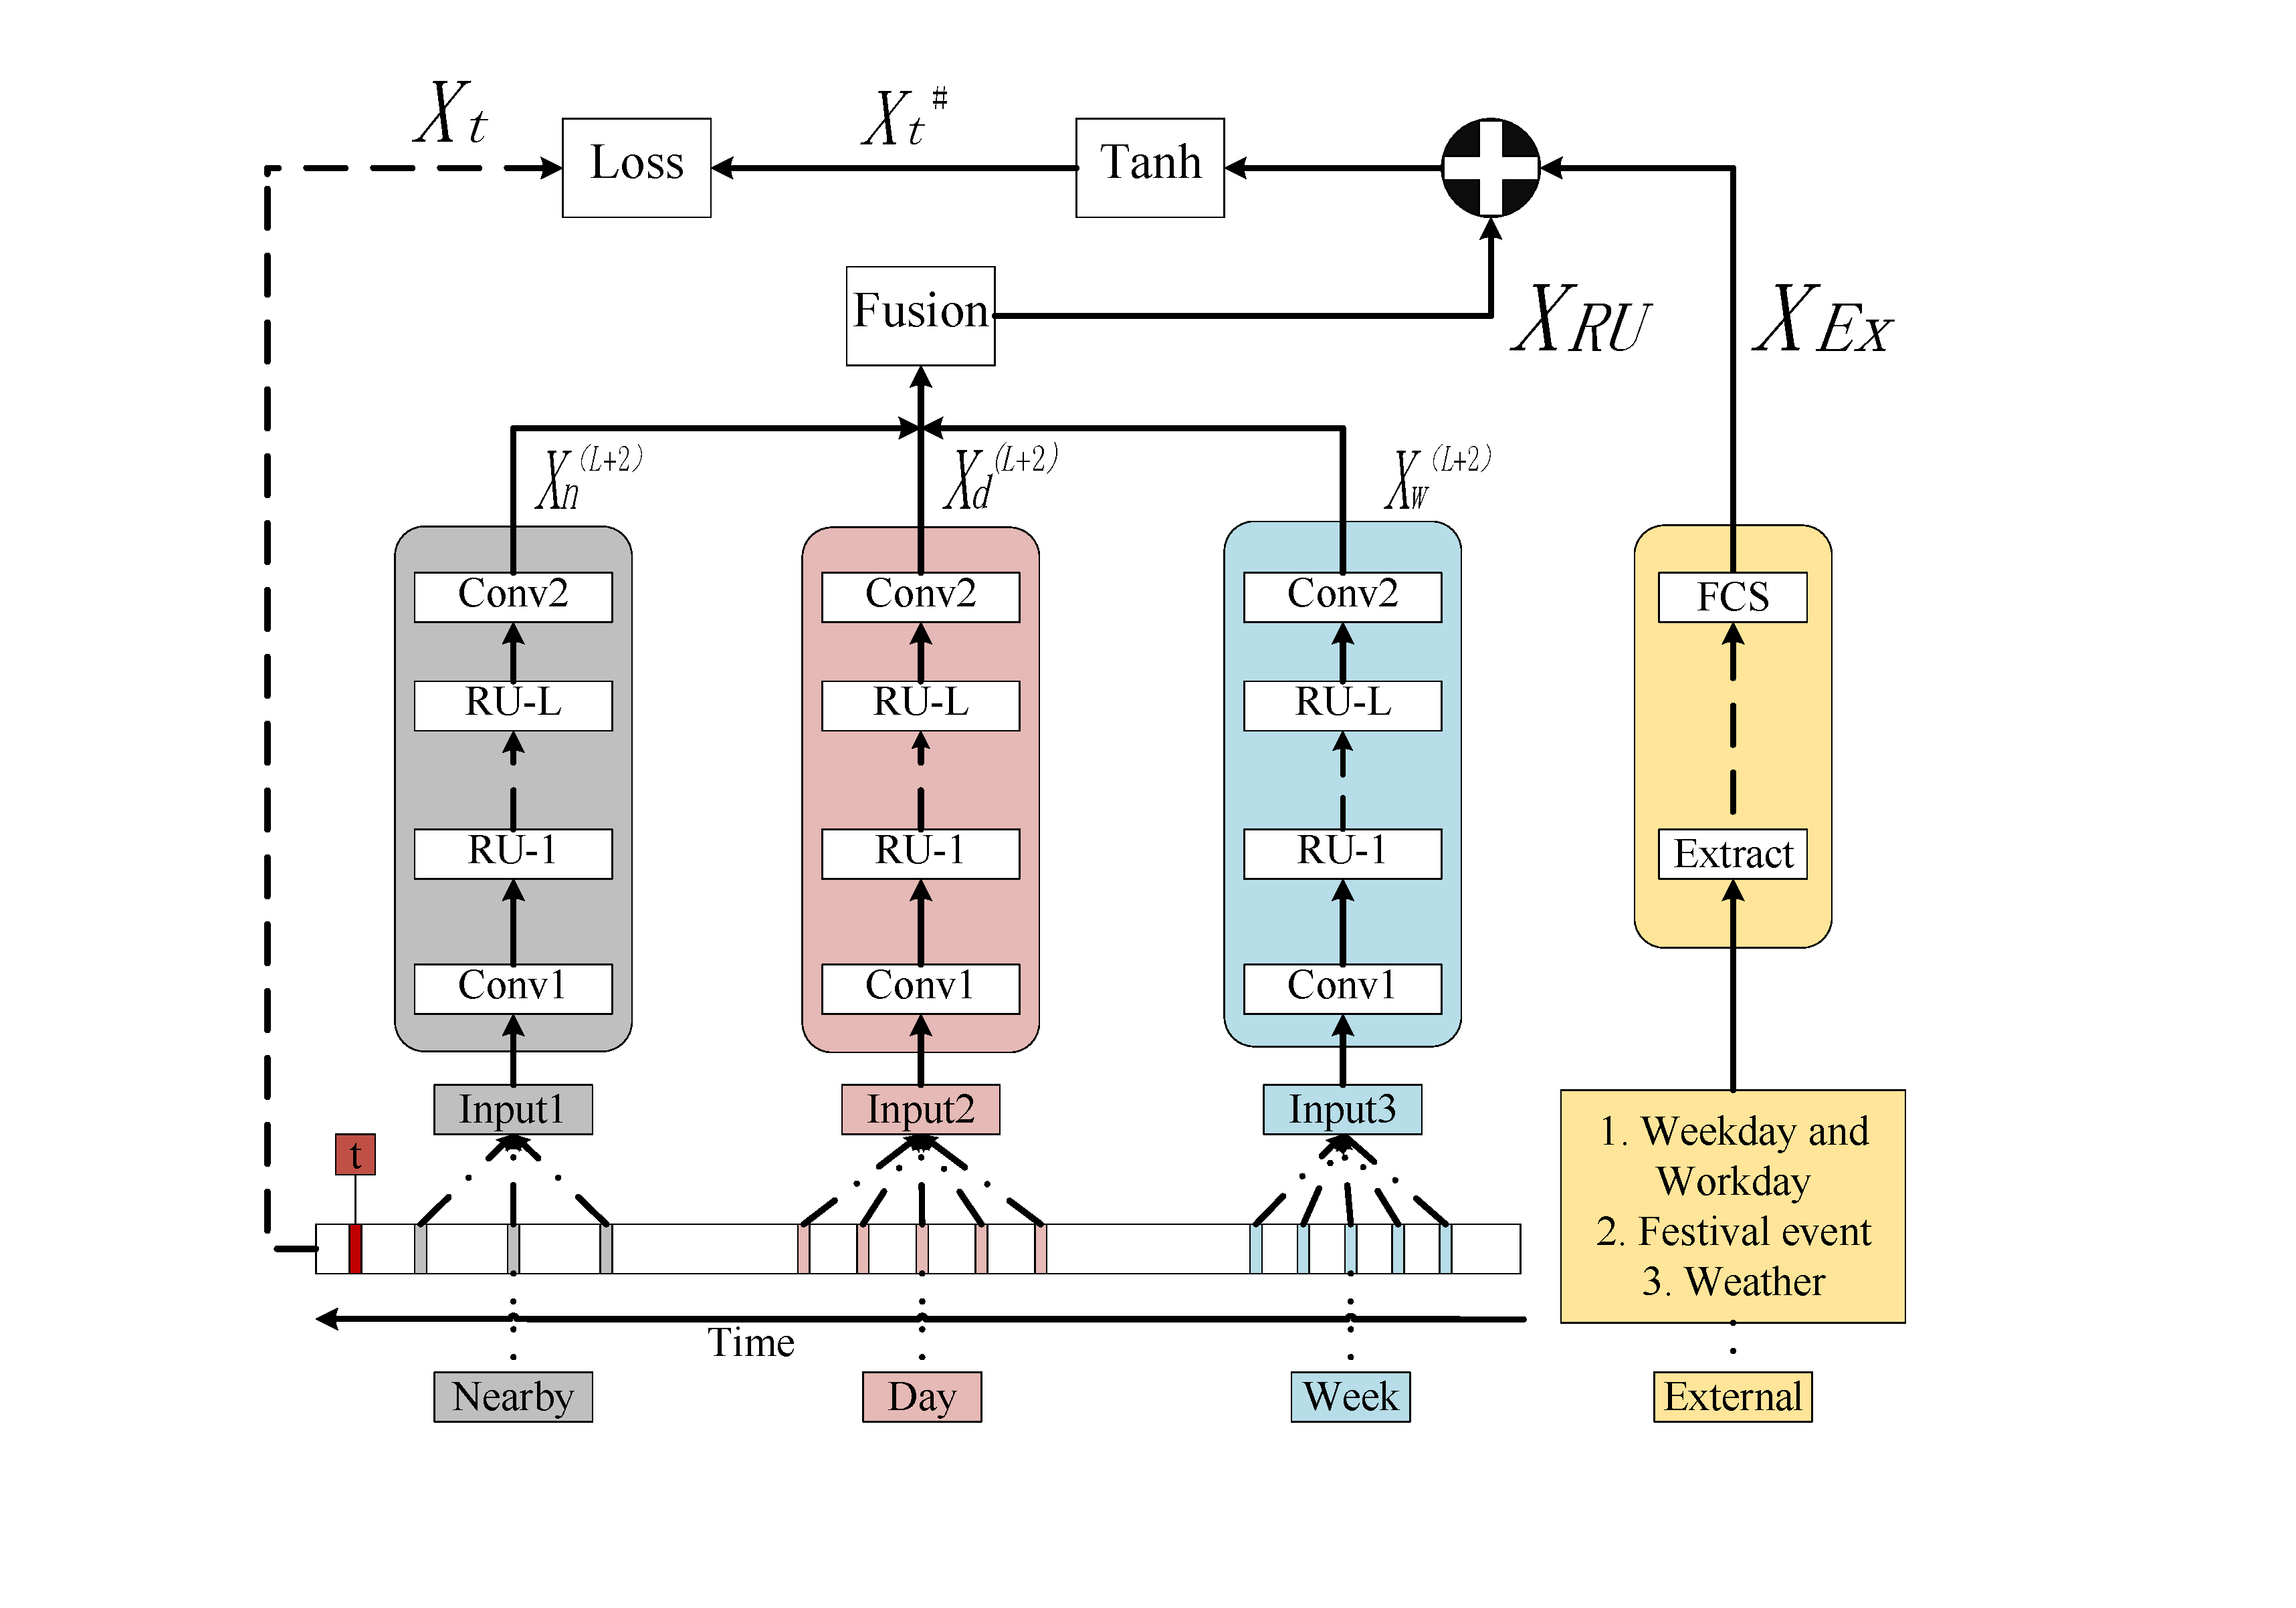
\includegraphics[width=9cm]{model.pdf}}
\caption{The structure of ST-DRN. Conv:one-dimensional convolution; RU:residual unit; FC:fully-connected}
\label{fig1}
\end{figure}

\subsection{Crowed Flows in Metro Station}
In this study, we predict inflow and outflow of all metro stations in a city, as shown in Fig.~\ref{fig3}, based on a sequence in all subway lines�� stations placed into an array K one by one. We partition a record in AFC system, the format of it in Table \uppercase\expandafter{\romannumeral1}, into an inflow and outflow depended on the in information (i.e. In\underline{ }date, In\underline{ }station and In\underline{ }time) and out information (i.e. Out\underline{ }date, Out\underline{ }station and Out\underline{ }time). As in before 6:00 and after 23:00, closing the time to start and stop of subway train in city, most of stations have no crowd flows, in the paper, we predict the flow from 6:00 to 23:00 and use 30 minutes as a time slot. And it��s also possible for no flows in a station that we fill zero as the flows number for training or testing ST-DRN model. After preprocessing, we show the number of statistics using half hour as a slot in one station at January 2017 in Table \uppercase\expandafter{\romannumeral2}.
=======
\item We evaluate our approach using Suzhou AFC subway system record data. The results demonstrate the advantages of our approach compared with some baselines. Furthermore, considering the data collected not be timely, we propose using data of earlier one hour than predicted time t and only adjust the parameters of nearby, day and week to indicate our model practical value on real subway system.
\end{itemize}

\section{Related Work}
In this section, we briefly definite the crowd flow for a station with the data format collected by AFC in Suzhou subway system and introduce deep residual learning.
\subsection{Crowed Flows in Metro Station}
>>>>>>> bd017bd6b8aa7e5822fa100cfe12d52184bfedc4
\begin{table}[htbp]
\caption{Data format in Suzhou metro card record}
\begin{center}
\begin{tabular}{|c|c|c|c|}
\hline
<<<<<<< HEAD
Card\underline{ }no& In\underline{ }date& In\underline{ }station& In\underline{ }time \\
=======
Care\underline{ }no& In\underline{ }date& In\underline{ }station& In\underline{ }time \\
>>>>>>> bd017bd6b8aa7e5822fa100cfe12d52184bfedc4
\hline
1& 2& 3& 4 \\
\hline
Out\underline{ }date& Out\underline{ }station& Out\underline{ }time&  \\
\hline
5& 6& 7&  \\
\hline
\end{tabular}
\label{tab1}
\end{center}
\end{table}

<<<<<<< HEAD
The inflow and outflow in all K stations can be represented as a tensor $X_t\in\mathnormal{R}^{K\times2}$ where $\left(X_t\right)_{k,0}=x_t^{k,in}$, $\left(X_t\right)_{k,1}=x_t^{k,out}$ at the $t^{th}$ time slot. For this dynamic system over a spatial station point denoted by array K, there are inflow and outflow at each station point over each time slot. Thus the data mined by us to be a format $X\in\mathnormal{R}^{K\times2}$ tensor at any time. And given the historical data $\{X_t|t=0,...,i-1\}$, in this paper, we forecast $X_t$ by using different time slot data.

\subsection{Residual Unit}
As we all well known, large deep convolutional networks compromise training effectiveness though the outstanding activation function (e.g. ReLU) and regularization techniques are utilized \cite{2,11}. And we still need a deep network to tackle very large metro stations dependencies, specially if the number of station is large in a city. For metro stations' flows data of a city, typically, presume that the number of stations is 59 , and the kernel size of one-dimensional convolution is used to 40, different size with different performance of model depending on the length of most people taking subway time  and stations' layout in a city as we use one-dimensional convolution. If we want to capture all metro stations' dependencies (i.e., each node in high-level layer depends on all nodes of the input), it needs more than 10 succeeding convolutional layers. To handle this problem, we apply residual learning \cite{1} in model, showing very effective for training super deep neural networks of more than 1000 layers.
=======
In this study, we predict inflow and outflow of all metro stations in a city, as shown in ''Fig. \ref{fig3}'', based on a sequence in all subway lines�� stations sorted into an array K one by one. We partition a record in AFC system, the format of it in Table \uppercase\expandafter{\romannumeral1}, into an inflow and outflow. As in before 6:00 and after 23:00, closing the time to start and stop of train in city, most of stations have no crowd flows, in the paper, we predict the flow from 6:00 to 23:00 and use 30 minutes as a time slot. And it��s also possible for no flows in a station that we fill zero as the flows number for training or testing ST-DRN model.

The inflow and outflow in all K stations can be represented as a tensor $X_t\in\mathnormal{R}^{K\times2}$ where $\left(X_t\right)_{k,0}=x_t^{k,in}$, $\left(X_t\right)_{k,1}=x_t^{k,out}$ at the $t^{th}$ time slot. For this dynamic system over a spatial station point denoted by array K, there are inflow and outflow at each station point over each time slot. Thus the data mined by us to be a format $X\in\mathnormal{R}^{K\times2}$ tensor at any time. And given the historical data $\{X_t|t=0,...,i-1\}$, in this paper, we forecast $X_t$ by using different time slot data.


\subsection{Deep Residual Learning}
Deep residual learning \cite{1} allows convolution neural networks to have ultra-deep structures in excess of 100 layers, even over 1000 layers, still displaying compelling accuracy and convinced convergence behaviors. Furthermore this method has shown compelling results on diverse challenging identification tasks, including image classification, object detection, segmentation and localization \cite{1}.

In formal, a residual unit \cite{3} with an identity mapping is defined as:
\begin{equation}
X^{(l+1)}=X^{(l)}+F\left(X^{(l)}\right)\label{1}
\end{equation}

where $X^{(l)}$ and $X^{(l+1)}$ are the input and output of the $l^{th}$ residual unit, respectively;  F is a residual function, e.g., a stack of two $3\times3$ convolution layers \cite{3}.  The core idea of the residual learning is to learn the additive residual function F with respect to $X^{(l)}$ \cite{3}.

\section{ST-DRN Model}

 ''Fig. \ref{fig1}'' display the structure of ST-DRN model, which is consisted of four main parts modeling nearby, day, week and external elements, respectively. As demonstrated in ''Fig. \ref{fig1}'', first we translate Inflow and outflow throughout all city metro subway system station at each time interval into a 2-channel array-like tensor, using the method introduced in above. Then we divide the time axis into three segments before the predicted time, representing nearby effects, day history and week history. Next the 2-channel flow tensors of slots in each time segment are fed into the first three parts, sharing the same network structure with a one-dimensional convolutional neural network allowed by a Residual Unit sequence, respectively to model the before mentioned three temporal factors: nearby, day and week, separately. This structure captures the spatial dependency between nearby and distant stations by one-dimensional convolution. In the external component, we manually collect some features from external data sets, such as holidays, weather conditions and workday or weekend, feeding them into a two-layer fully-connected neural network. The results of the first three parts are fused as $X_{RU}$ based on parameter matrices, which assign different weights to the outputs of different components in different parts. $X_{RU}$ is further combined with the output of the external component $X_{Ex}$. In the end, the integration is mapped into [-1, 1] by a Tanh function, which yields a faster convergence than the standard logistic function in the process of back-propagation learning \cite{5}. In the next some subsections, we give the evidence to prove the spatial, temporal and external influence to the station crowed flows.

\begin{figure}[htbp]
\small
\centerline{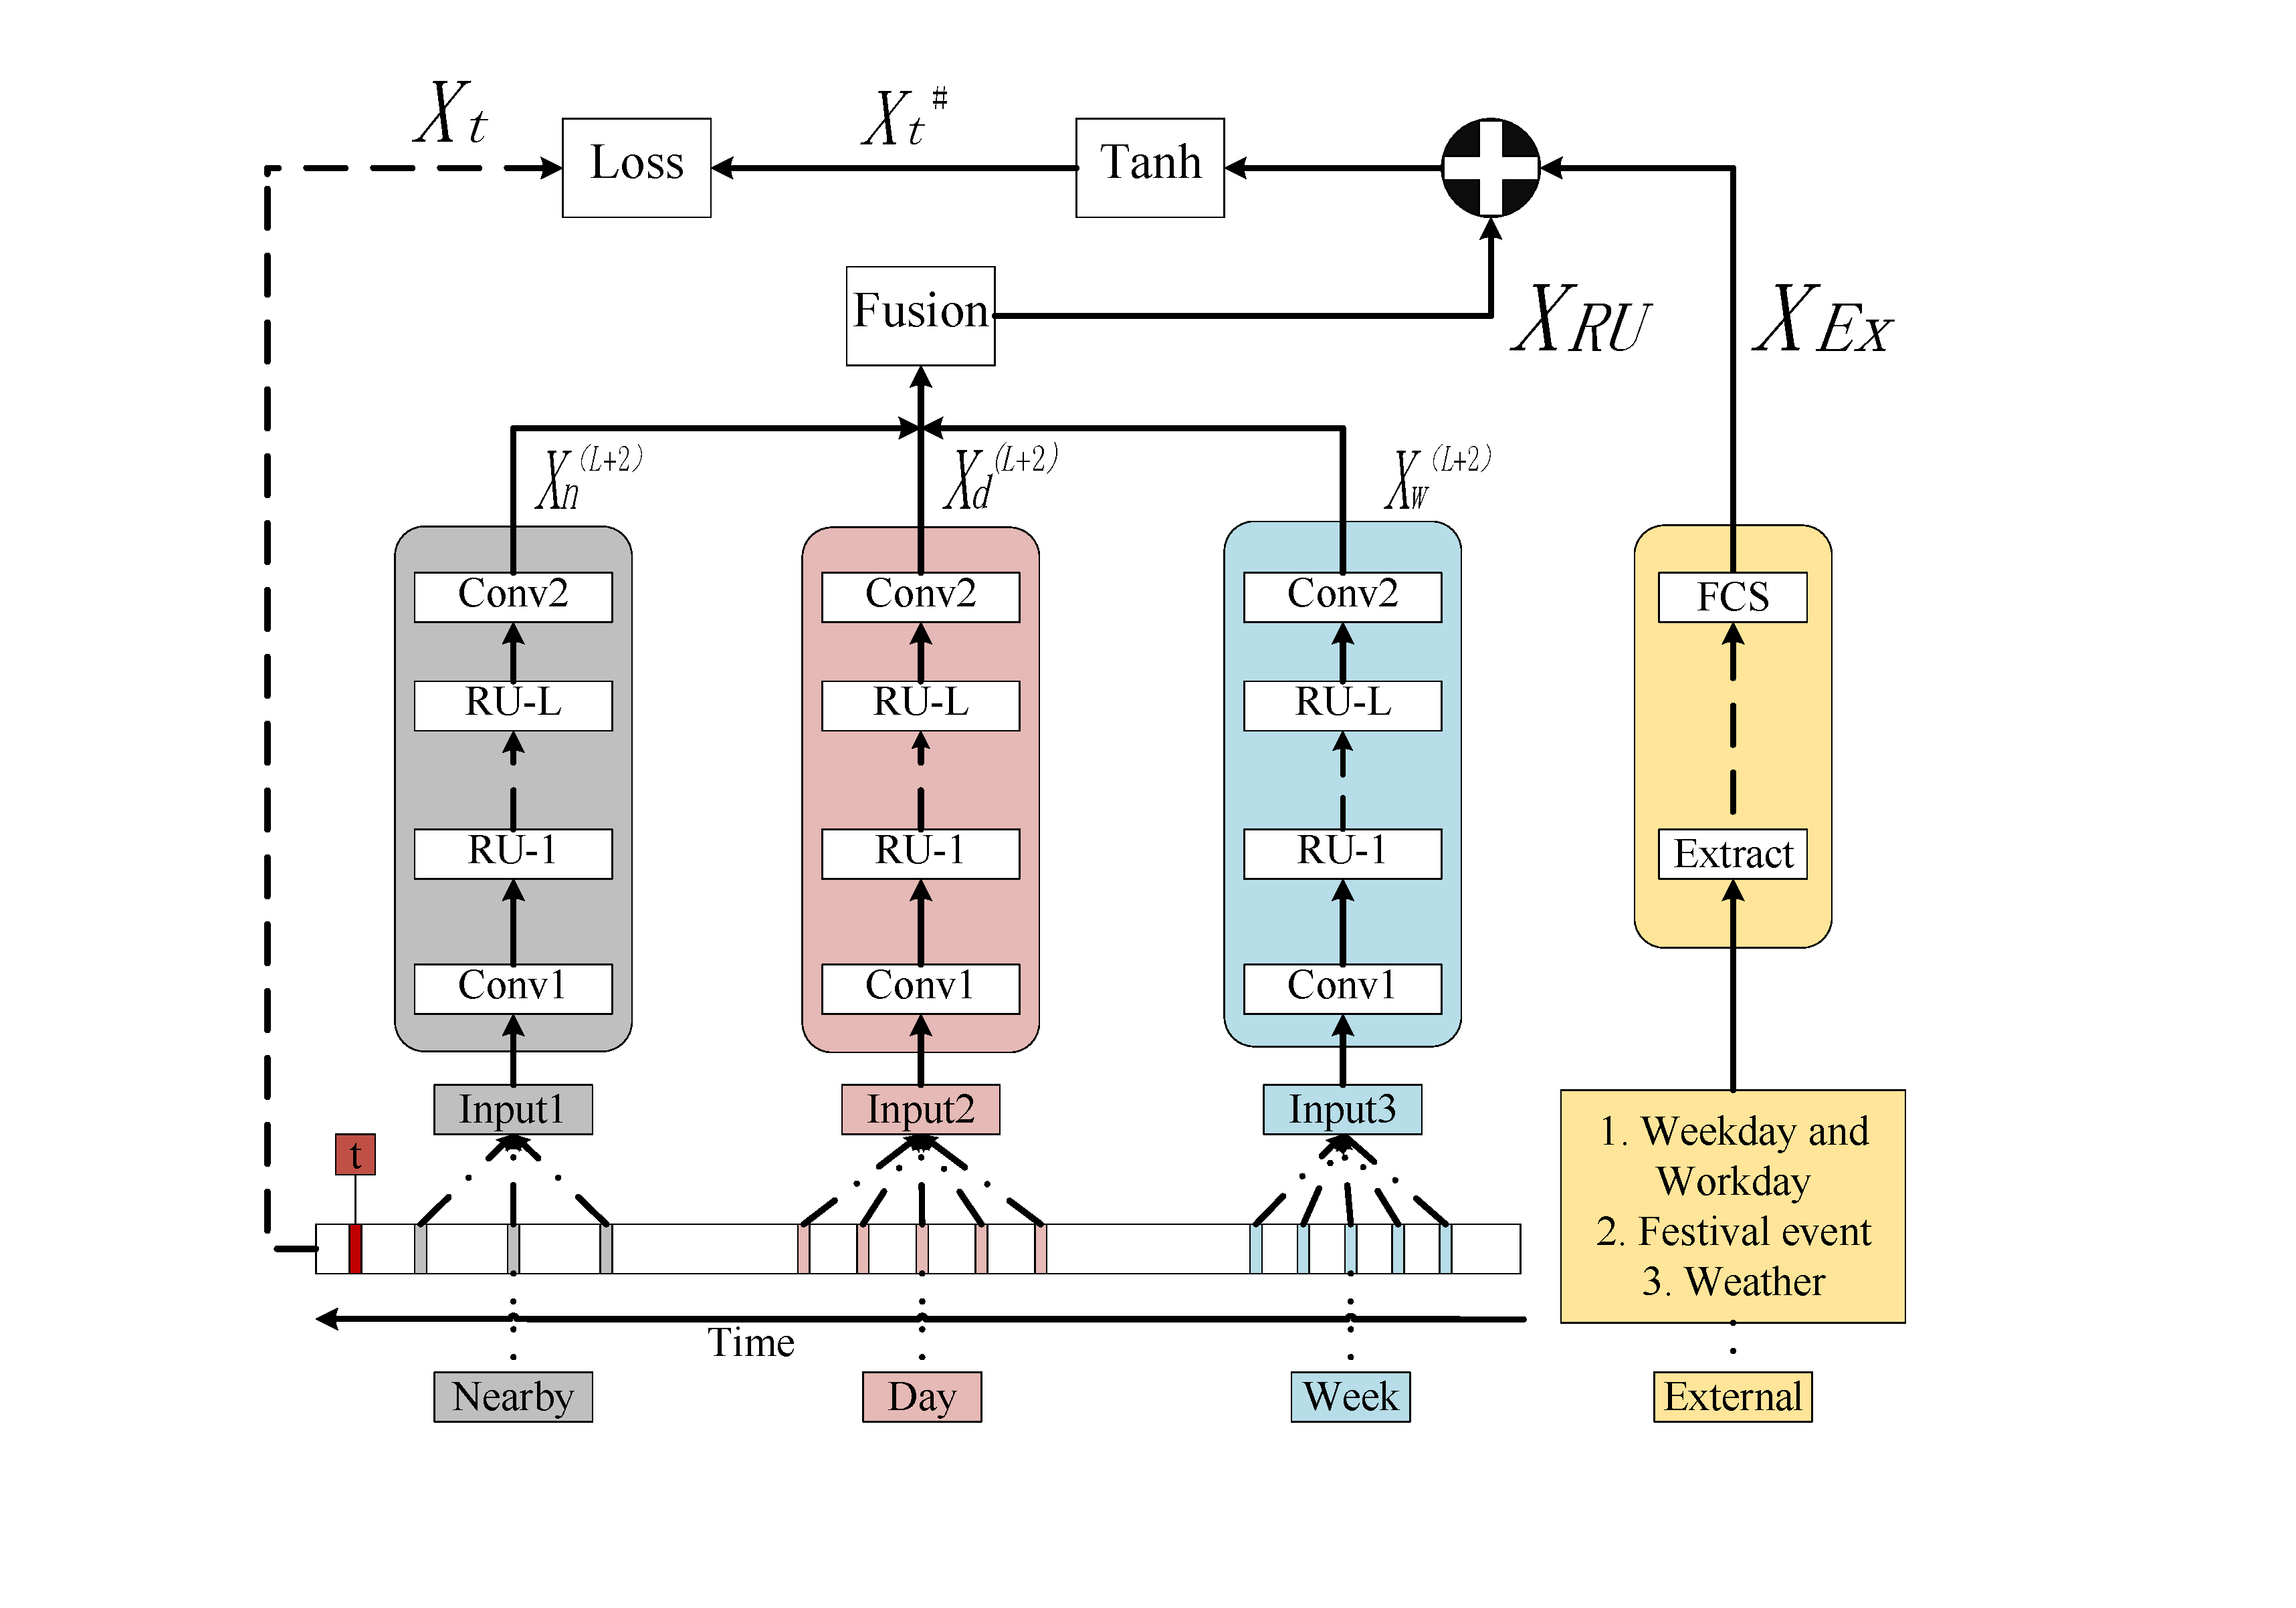
\includegraphics[width=9cm]{model.pdf}}
\caption{The structure of ST-DRN. Conv:one-dimensional convolution; RU:residual unit; FC:fully-connected}
\label{fig1}
\end{figure}

\subsection{Residual Unit}
As we all well known, large deep convolutional networks compromise training effectiveness though the outstanding activation function (e.g. ReLU) and regularization techniques are utilized \cite{2,11}. And we still need a deep network to tackle very large metro stations dependencies, specially if the number of station is large in a city. For a metro stations flows data, typically, presume that the number of stations is 59 , and the kernel size of one-dimensional convolution is used to 40, different size with different performance of model depending on the length of most people taking subway time  and stations' layout in a city as we use one-dimensional convolution. If we want to capture all metro stations' dependencies (i.e., each node in high-level layer depends on all nodes of the input), it needs more than 10 succeeding convolutional layers. To handle this problem, we apply residual learning \cite{1} in model, showing very effective for training super deep neural networks of more than 1000 layers.
>>>>>>> bd017bd6b8aa7e5822fa100cfe12d52184bfedc4

\begin{figure}[htbp]
\small
\centerline{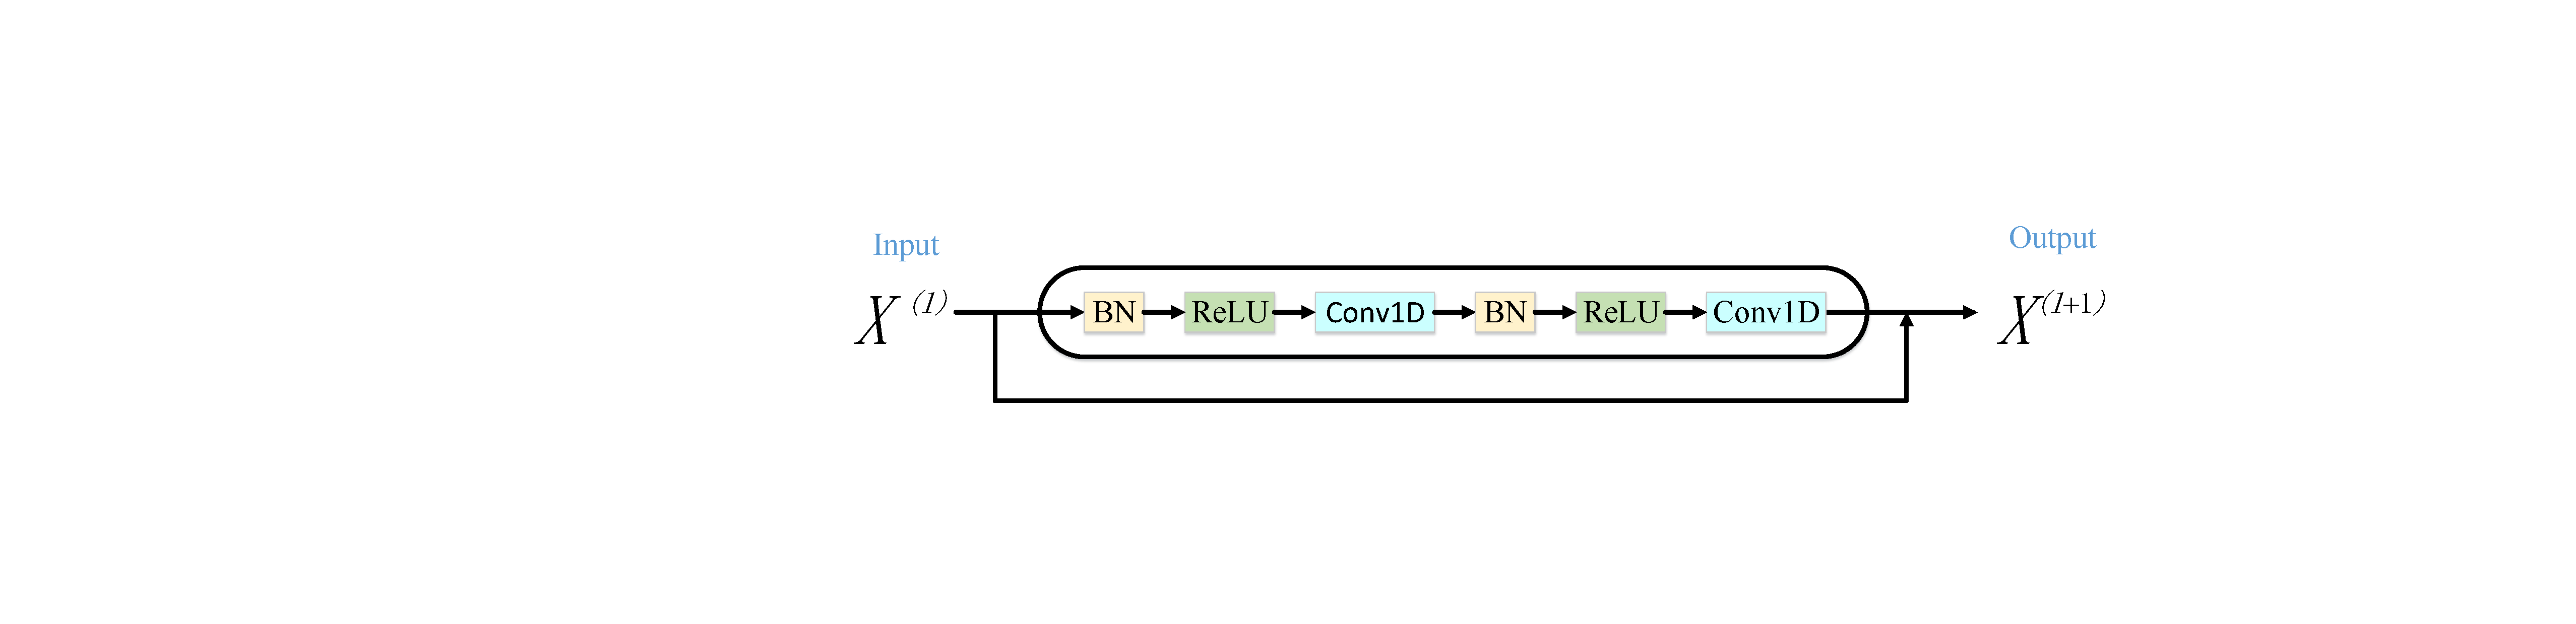
\includegraphics[width=9cm]{unit.pdf}}
\caption{Residual Unit; BN: batch normalization; ReLU: activation function; Conv1D: one-dimensional convolution}
\label{fig2}
\end{figure}

Residual Unit Function and equation:
\begin{equation}
X^{(l+1)} = X^{(l)} + F\left(X^{(l)};\theta^{(l)}\right), l=1,\cdots, L\label{2}
\end{equation}
<<<<<<< HEAD
where F is the residual function (i.e. consists of ��ReLU + Convolution��, see F in Fig.~\ref{fig2}), and $\theta^{(l)}$ includes all learnable parameters in the $l^{th}$ residual unit. We also employ Batch Normalization (BN) \cite{2} that is placed before ReLU, as shown in Fig.~\ref{fig2}.
=======
where F is the residual function (i.e. consists of ��ReLU + Convolution��, see F in ''Fig. \ref{fig2}''), and $\theta^{(l)}$ includes all learnable parameters in the $l^{th}$ residual unit. We also employ Batch Normalization (BN) \cite{2} that is placed before ReLU, as shown in ''Fig. \ref{fig2}''.
>>>>>>> bd017bd6b8aa7e5822fa100cfe12d52184bfedc4
\subsection{Spatio Elements}
A city usually has a very large size, containing many metro stations with different distances. Intuitively, the inflow of crowds in a station may affect other stations' outflow depending on the most of people taking ride time length, which can be effectively processed by the convolutional neural network (CNN) that has shown its powerful ability to hierarchically handle the spatial structural information \cite{5}. Furthermore, subway systems connect two stations with a very far distance, leading to the dependency between distant stations. In order to process the spatial dependency of any station, we need to construct a CNN with many layers because one convolution only handling spatial near dependencies, delimited by the size of their kernels. The same issue also has been found in the video sequence generating task where the input and output have the same resolution \cite{6}. Several methods have been introduced to avoid the loss of resolution brought about by sub-sampling while preserving distant dependencies \cite{12}. Different from the traditional CNN, we do not apply the sub-sampling (i.e. pooling), but only convolutions \cite{13}. We discover that a node in the high-level feature map depends on some nodes, relying on the size of convolution kernel, of the middle-level feature map, those of which depend on all nodes in the lower-level feature map (i.e. input). It means that one convolution naturally handles station near dependencies, and deep layers convolutions can further handle distant even all stations' dependencies.

\begin{figure}[htbp]
\small
<<<<<<< HEAD
\centerline{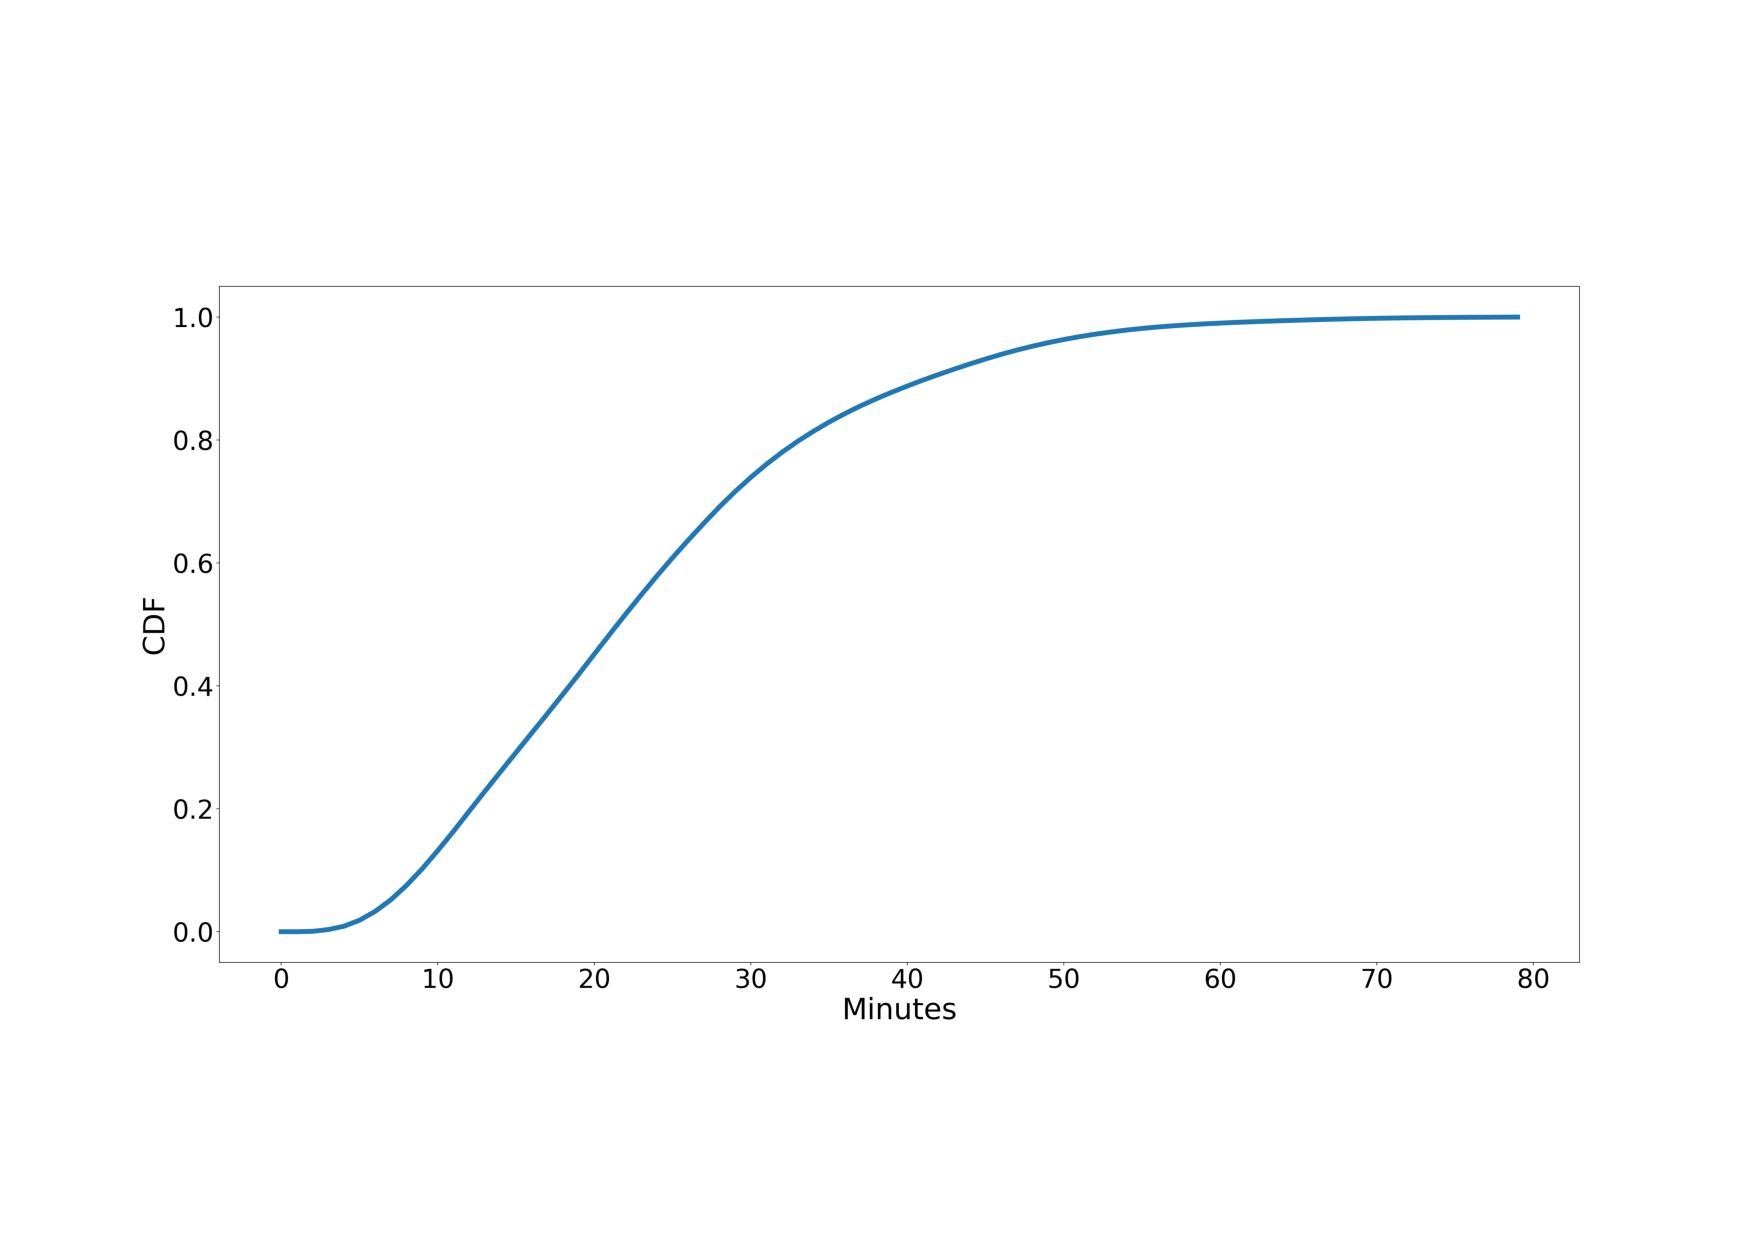
\includegraphics[width=9cm]{CDF.pdf}}
=======
\centerline{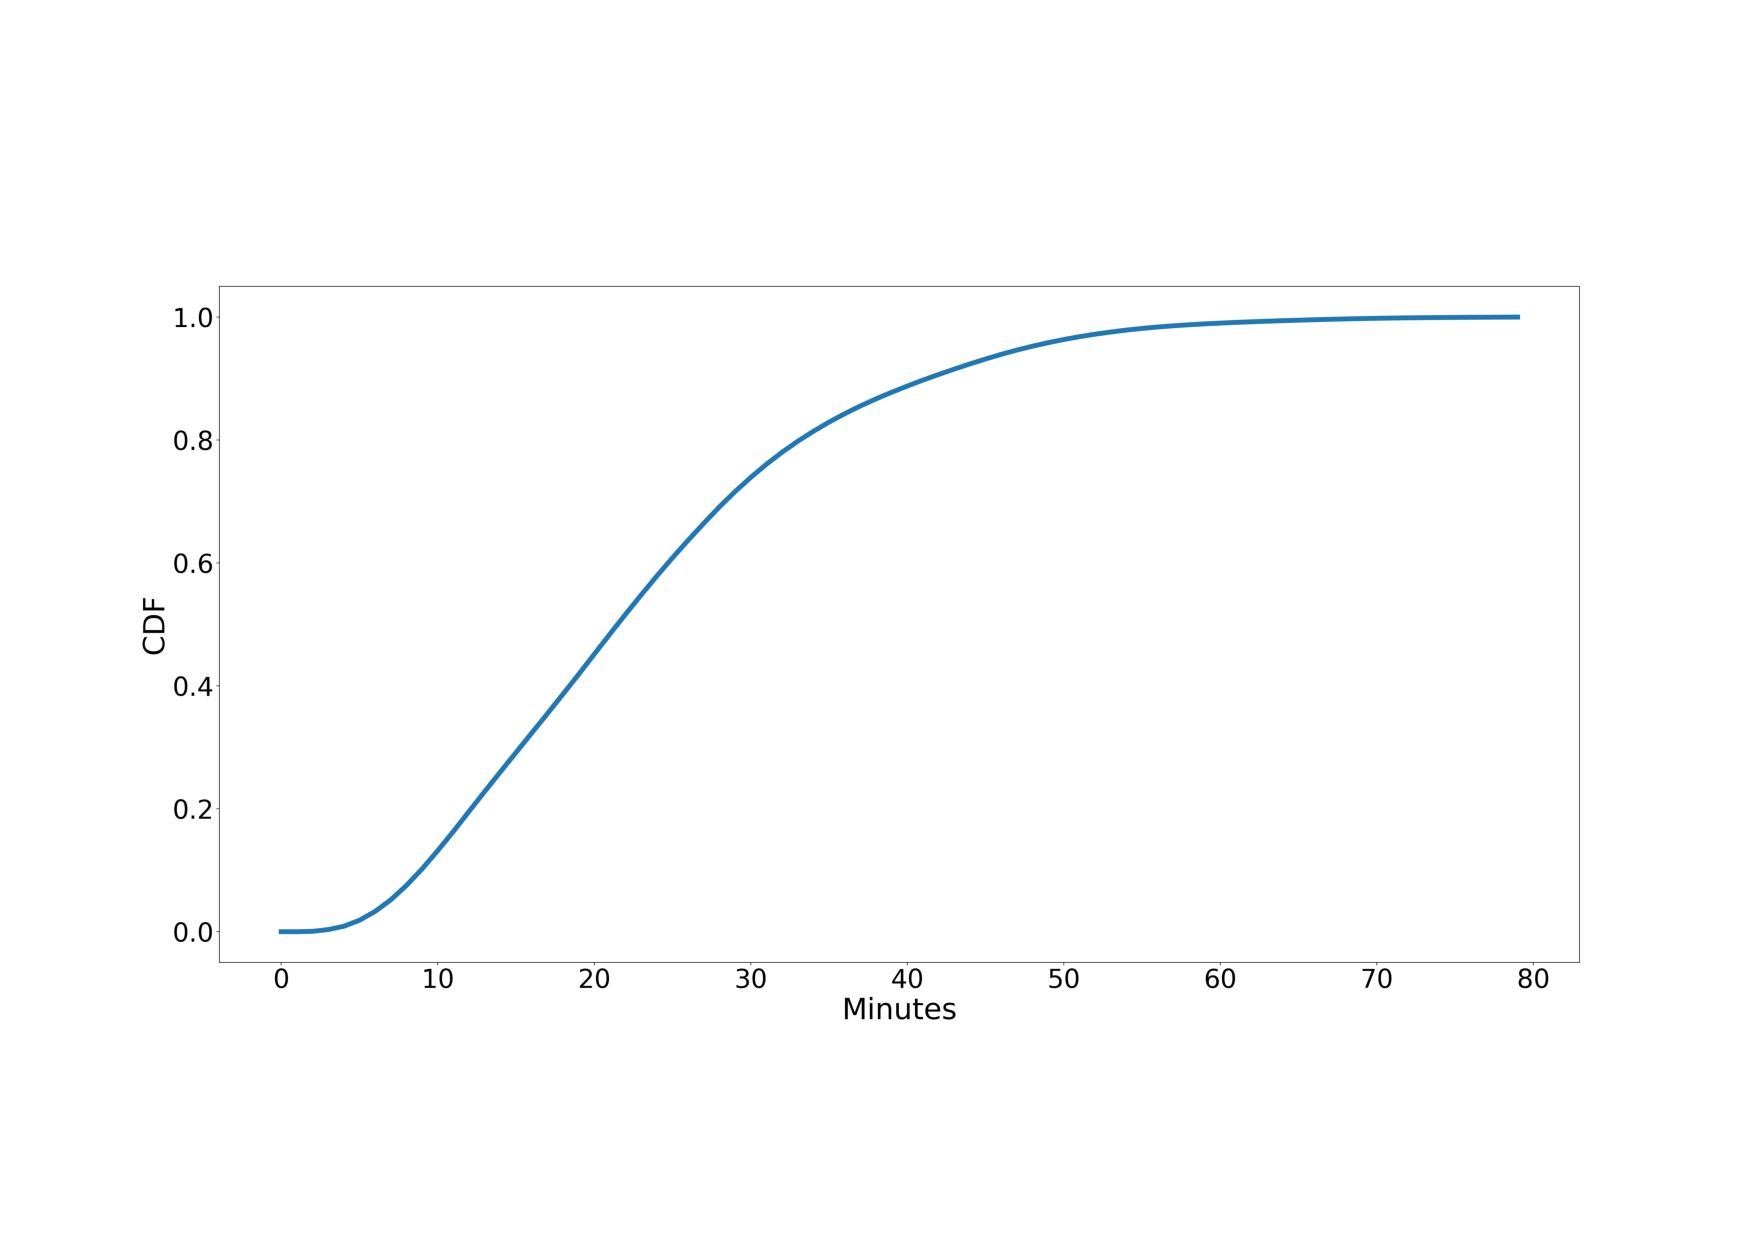
\includegraphics[width=6cm]{CDF.pdf}}
>>>>>>> bd017bd6b8aa7e5822fa100cfe12d52184bfedc4
\caption{CDF of taking ride time length in SuZhou (January 2017).}
\label{fig3}
\end{figure}

<<<<<<< HEAD
In this paragraph, we discuss how to chose the kernel size of one-dimensional convolution.  We draw the figure of metro stations distribution at Suzhou, Showing in Fig.~\ref{fig4}, and mark the number for each station, the cross station number the N-9 in line1 and number N-38 in line2. According to Fig.~\ref{fig3}, we can summary that the most taking ride time length range from 10 minutes to 40 minutes at Suzhou. Removing the waiting time and transferring time, the maximum number of passengers through the station number is about 18. Obviously, The direction for the max value of station number is boarding in N-0 and leaving in N-42, actually just pass 14 stations in spatial. Considering the waiting time and  transferring time, the average subway departure time length, we chose about 40 as the best kernel size. And we will give different length experiment results in evaluation part to prove our discussion.
=======
In this paragraph, we discuss how to chose the kernel size of one-dimensional convolution. According to ''Fig. \ref{fig3}'', we can summary that the most taking ride time length range from 10 minutes to 40 minutes at Suzhou. Removing the waiting train time and transferring time, possibly, the most passenger go through station number approximately under 18. We draw the figure of metro stations distribution at Suzhou, Showing in ''Fig. \ref{fig4}'', and mark the number for each station, the cross station number the N-9 in line1 and number N-38 in line2. Obviously, The direction for the max value of station number is boarding in N-0 and leaving in N-42, actually just pass 14 stations in spatial. As the 6 minutes transferring time, the average subway departure time length, we chose about 40 as the best kernel size. And we will give different length experiment results in evaluation part to prove our discussion.
>>>>>>> bd017bd6b8aa7e5822fa100cfe12d52184bfedc4

\begin{figure}[htbp]
\small
\centerline{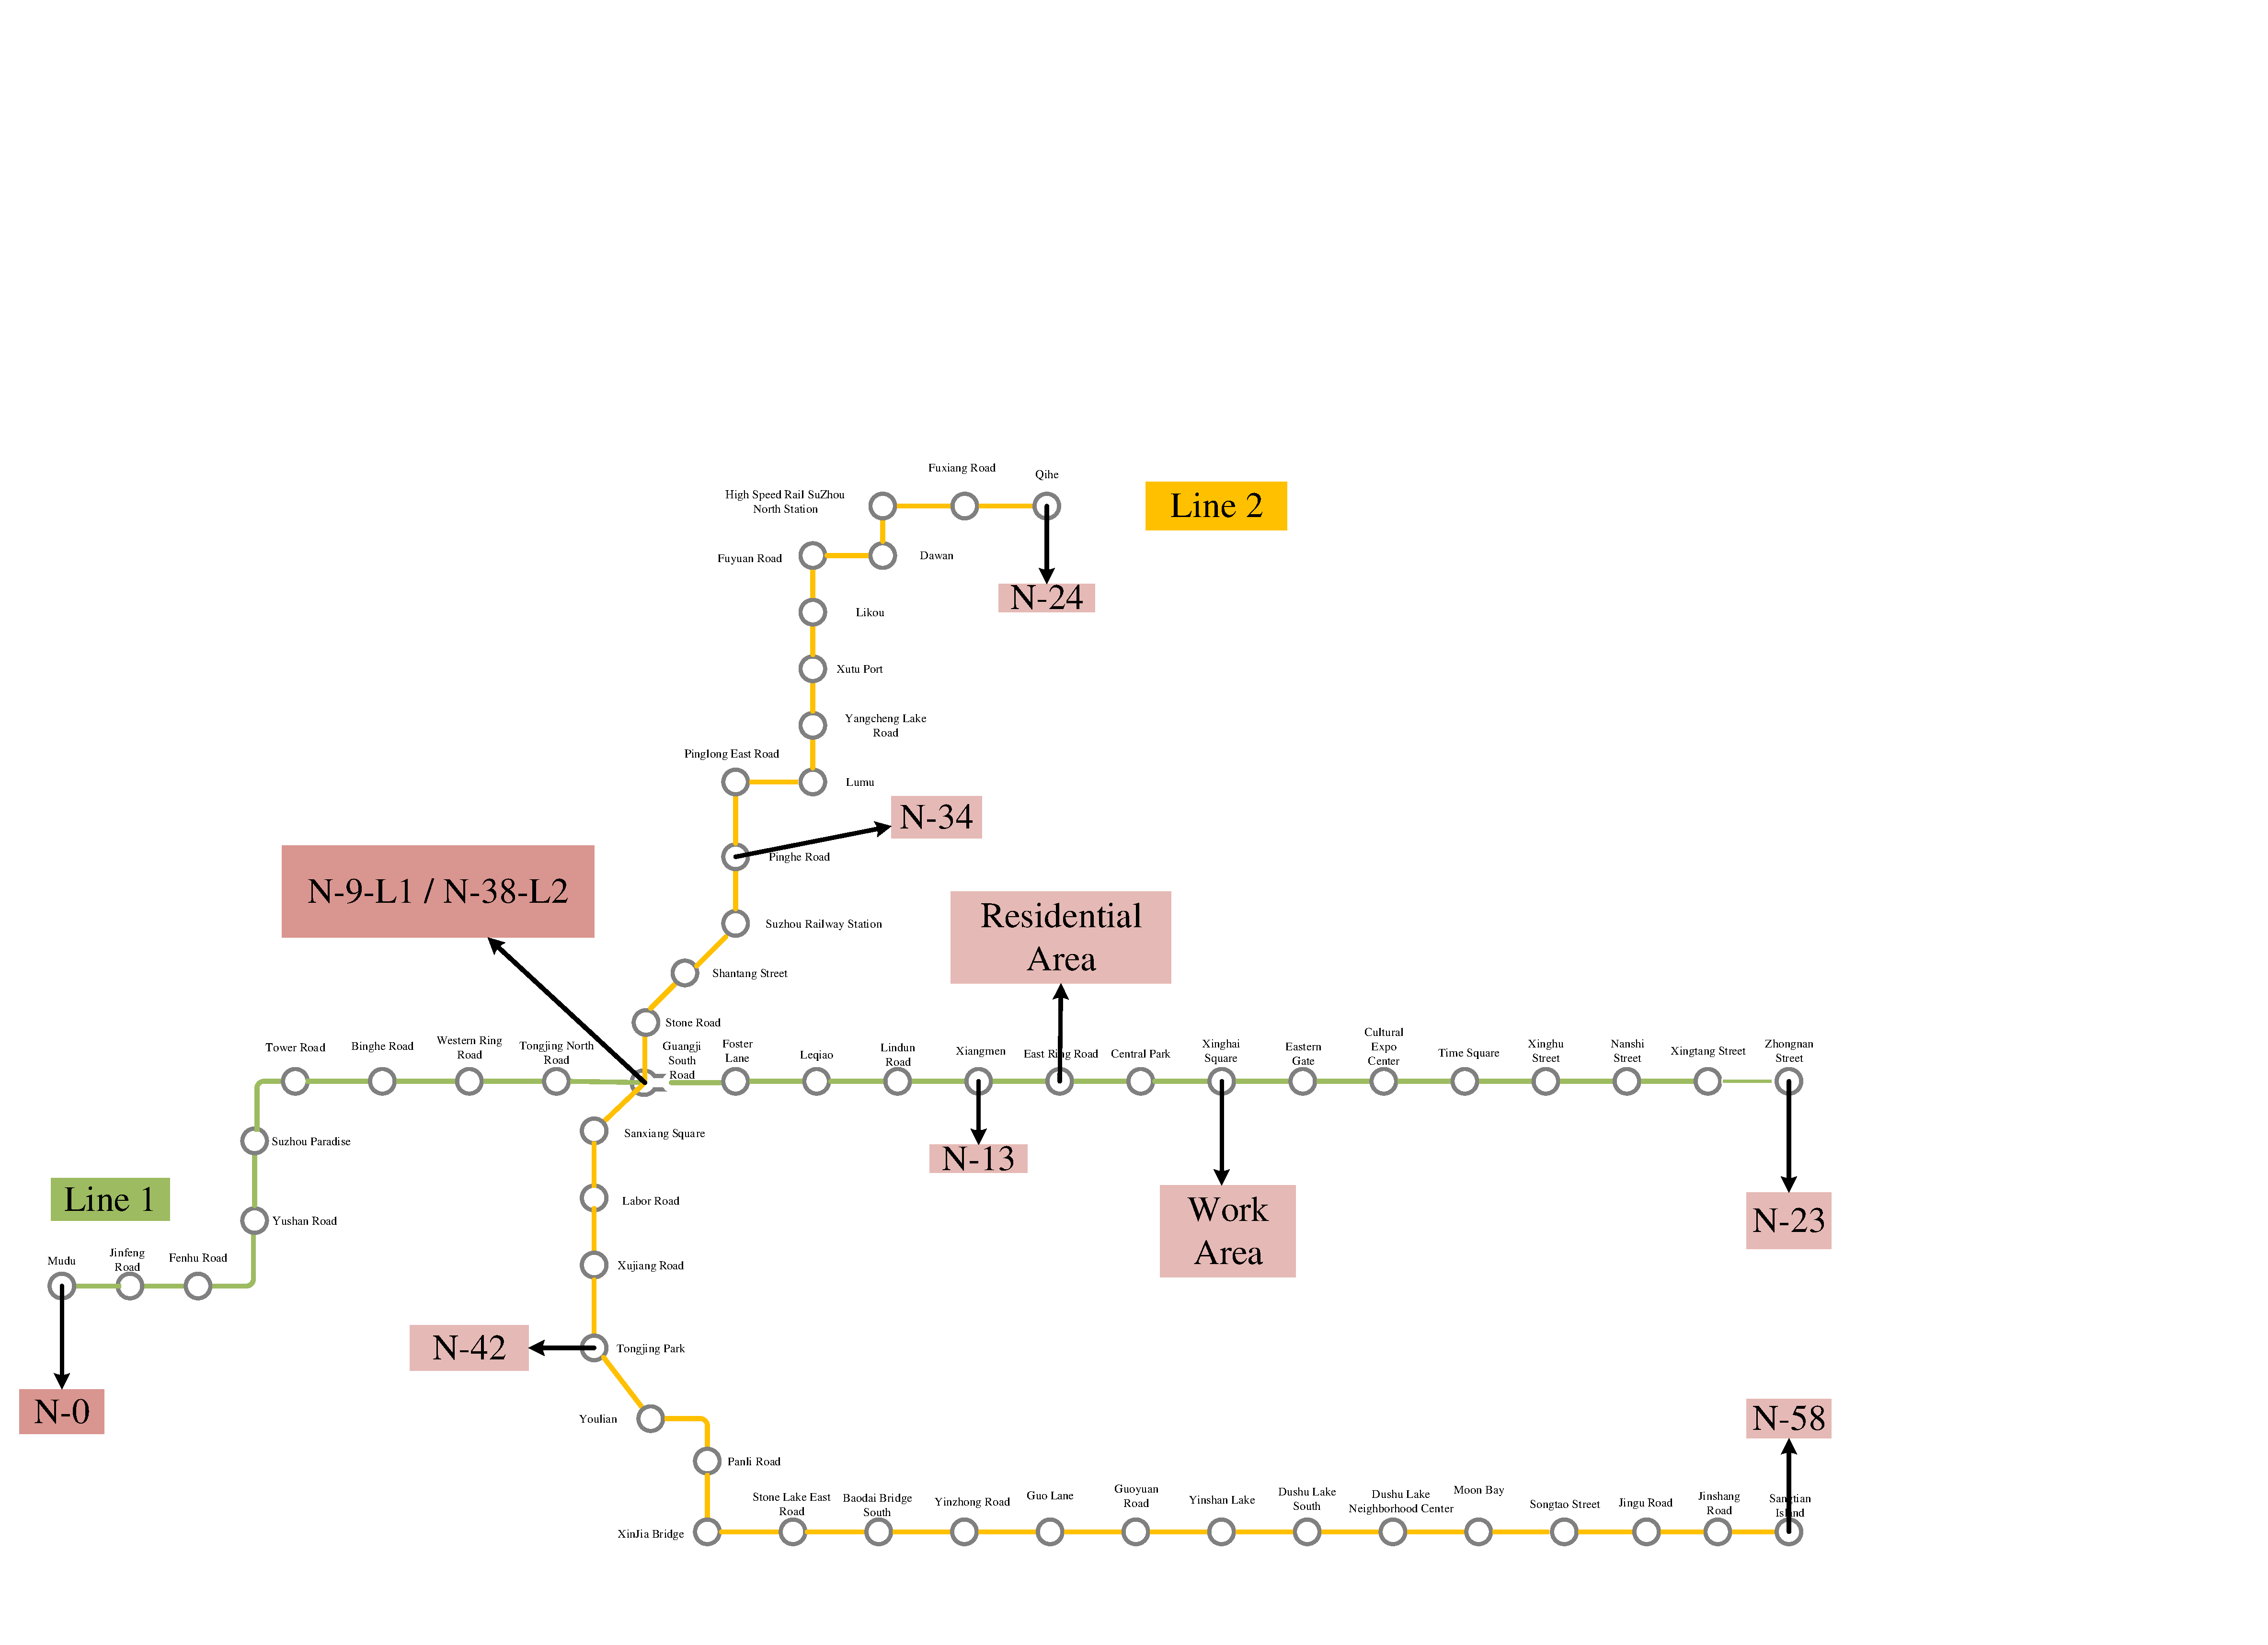
\includegraphics[width=9cm]{conv.pdf}}
\caption{The stations' distribution of Suzhou subway system.}
\label{fig4}
\end{figure}

\subsection{Temporal Elements}
<<<<<<< HEAD
\begin{figure*}[htbp]
\small
\centerline{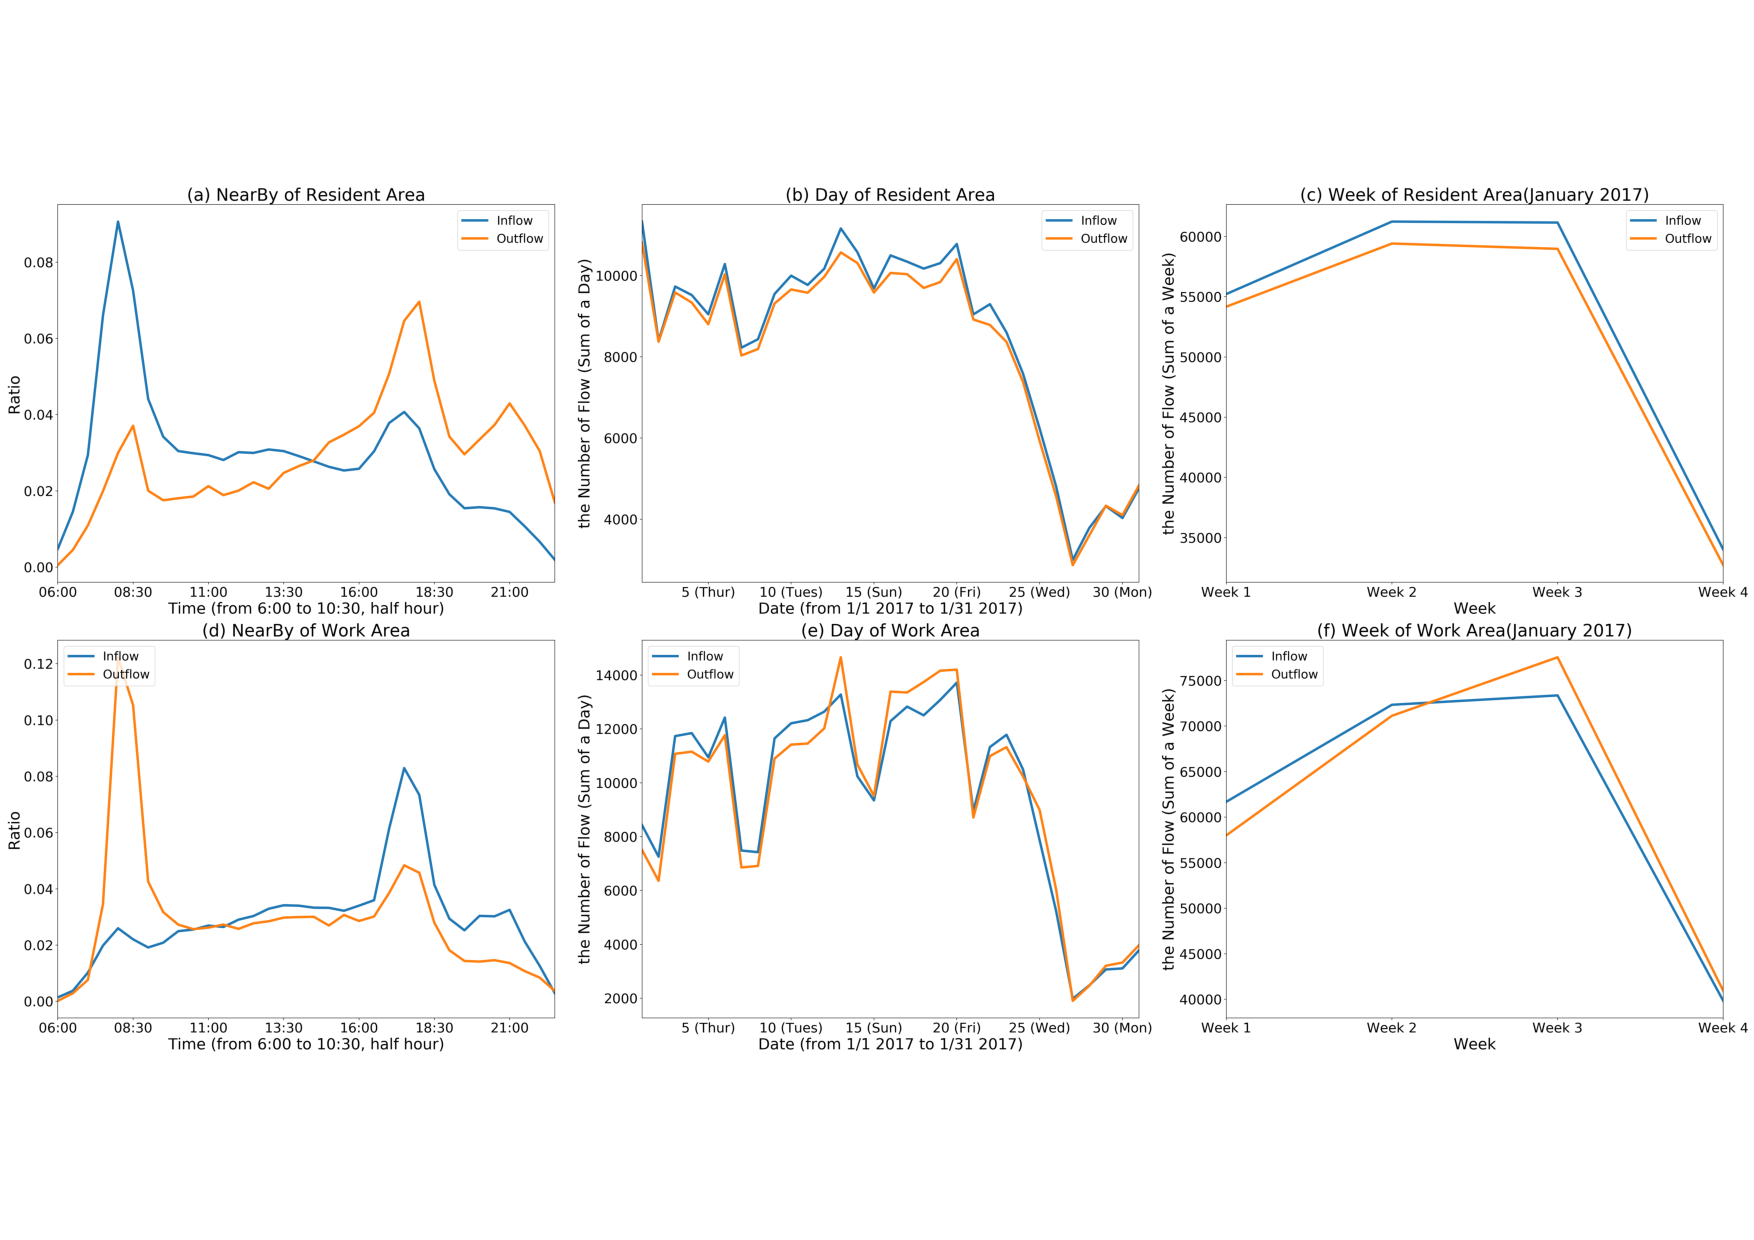
\includegraphics[width=18cm]{temporal.pdf}}
\caption{Temporal influences (Work Area and Residential Area are targeted in Fig.~\ref{fig3}).}
\label{fig5}
\end{figure*}
As shown in Fig.~\ref{fig1}, the first three parts (i.e. \emph{nearby}, \emph{day}, \emph{week}) share the same network structure, which is consisted of two sub-components: one-dimensional convolution and residual unit. Fig.~\ref{fig5} (a) and (d) show the ratio curves using Suzhou subway data presented in Table \uppercase\expandafter{\romannumeral2} where x-axis is time gap between two time slots and y-axis is the average ratio value between arbitrary two inflows at the same time gap. The curves from two different areas, marked in Fig.~\ref{fig4}, all show an empirical temporal conjunction in time series, in other words, inflows of close time slots are more relevant than ones of distant time slots, which implies temporal nearby. The two curves have different shapes, which demonstrates that different areas ave different features of nearby, particularly in morning and evening work peak. Fig.~\ref{fig5} (b) and (e) show flows at all time slots of 7 days. Distinctly we can see the daily periodicity in both areas, because of having trend fluctuation of week. In work area, the peak values on workdays are much higher than ones on weekends. Resident area has similar peak values for both workdays and weekends. Fig.~\ref{fig5} (c) and (f) describe sum of flows of one week at January 2017. As time goes by, the flows sharply decreases in work area and resident area, as the last week with Spring Festival, vary important for Chinese and many people moving from city serval days in advance. It shows the different trends in different areas. In conclusion, flows of this two areas are all influenced by \emph{nearby}, \emph{day}, and \emph{week}, but the extents of affect may be very different. This situation is also applicable to other stations.

The \emph{nearby} part in Fig.~\ref{fig1} employs a few 2-channel flows tensor of in slots prior the forecasting time, we want, to pattern temporal nearby dependence. Let the nearby segment be [$X_{t-l_n}$, $X_{t-(l_n-1)}$, \dots, $X_{t-1}$], called as the closeness dependent sequence. We first bind them along with the first axis (i.e. time interval) as one tensor $X_n^{(0)}\in\mathnormal{R}^{K\times2l_n}$, which is followed by a one-dimensional convolution (i.e. Conv1 shown in Fig.~\ref{fig3}) as:
=======
As shown in ''Fig. \ref{fig1}'', the first three components (i.e. nearby, day, week) share the same network structure, which is consisted of two sub-components: one-dimensional convolution and residual unit. ''Fig. \ref{fig5}'' (a) and (d) show the ratio curves using Suzhou subway data presented in Table \uppercase\expandafter{\romannumeral2} where x-axis is time gap between two time slots and y-axis is the average ratio value between arbitrary two inflows at the same time gap. The curves from two different areas, marked in ''Fig. \ref{fig4}'', all show an empirical temporal conjunction in time series, In other words, inflows of close time slots are more relevant than ones of distant time slots, which implies temporal nearby. The two curves have different shapes, which demonstrates that different areas ave different features of nearby, particularly in morning and evening work peak. ''Fig. \ref{fig5}'' (b) and (e) show flows at all time slots of 7 days. Distinctly we can see the daily periodicity in both Areas, because of having trend fluctuation of week. In work area, the peak values on workdays are much higher than ones on weekends. Resident area has similar peak values for both workdays and weekends. ''Fig. \ref{fig5}'' (c) and (f) describe sum of flows of one week at January 2017. As time goes by, the flows sharply decreases in work area and resident area, as the last week with Spring Festival, vary important for Chinese and many people moving from city serval days in advance. It shows the different trends in different areas. In conclusion, flows of this two areas are all influenced by nearby, day, and week, but the extents of affect may be very different. This situation is also applicable to other stations.

\begin{figure}[htbp]
\small
\centerline{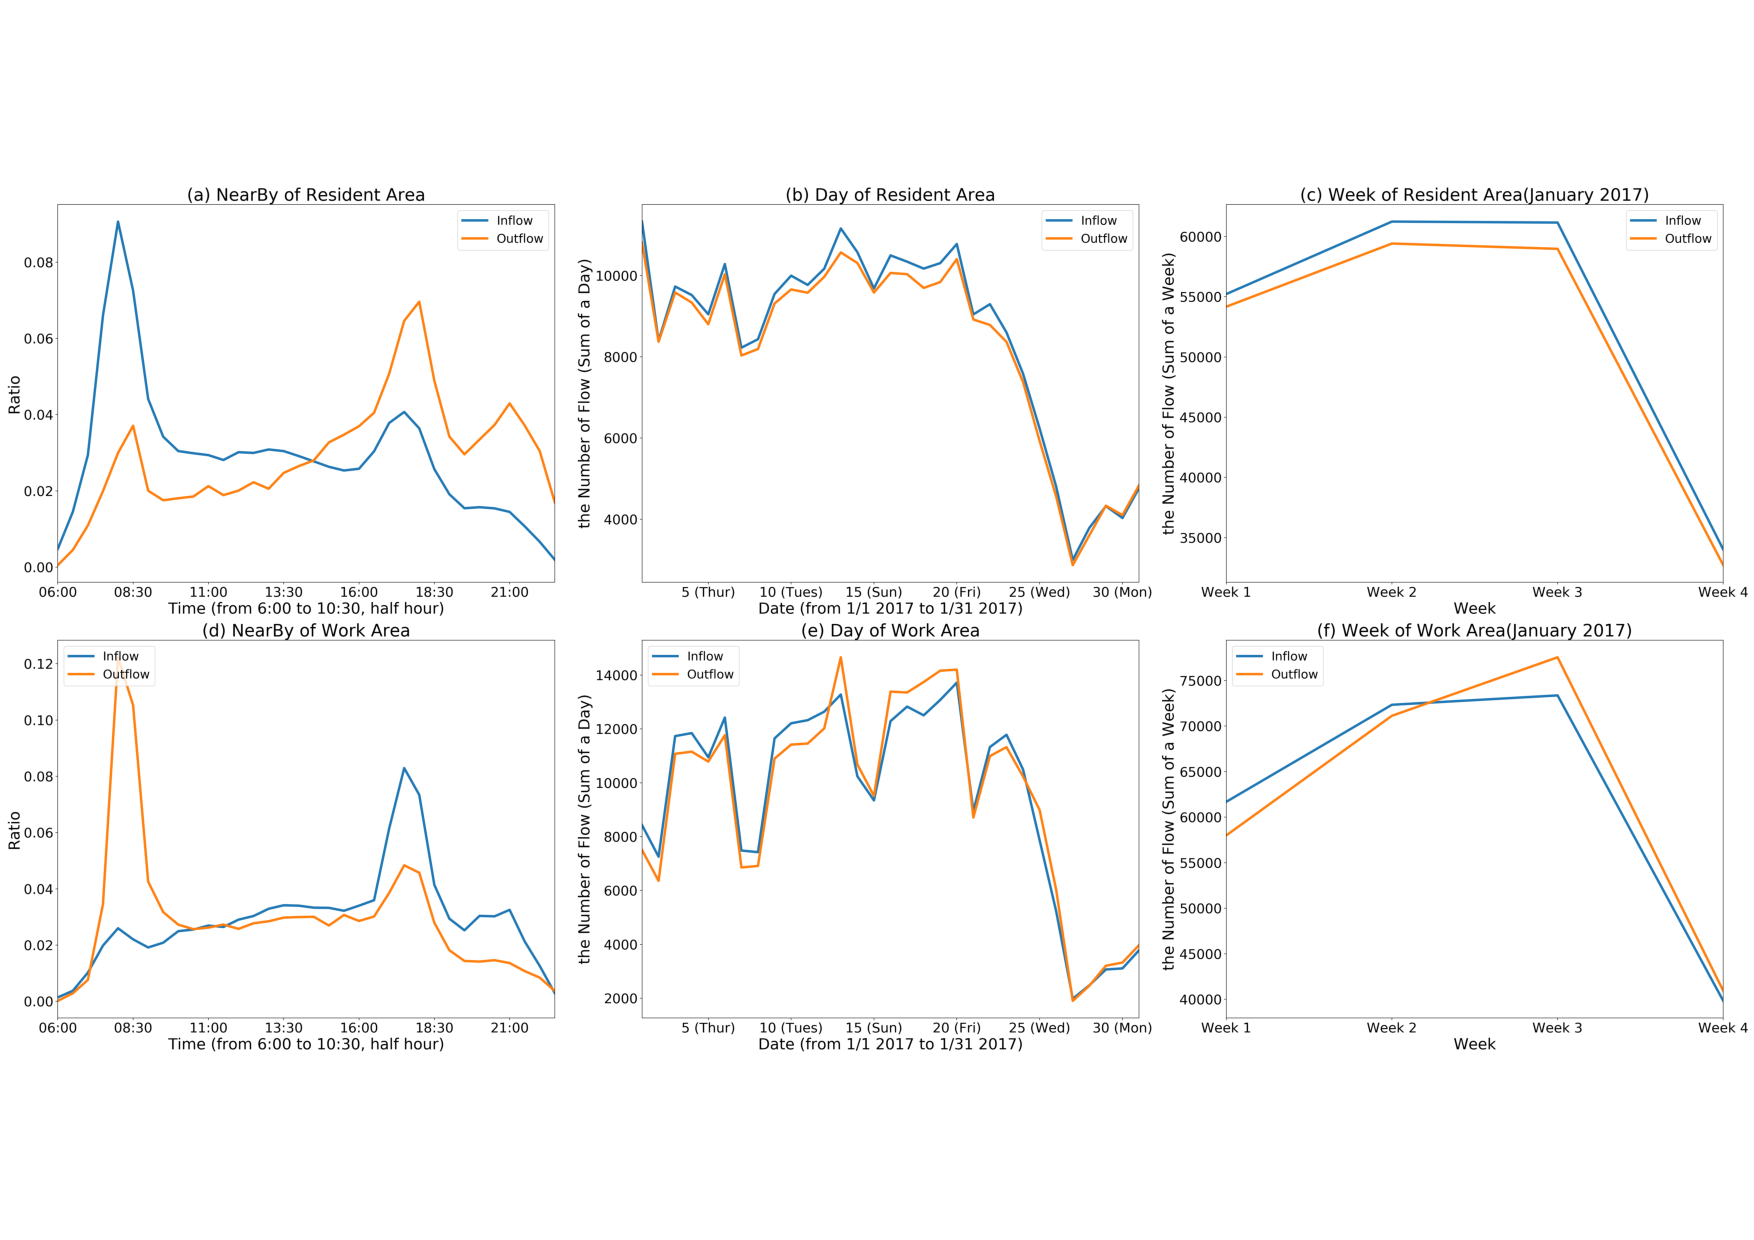
\includegraphics[width=9cm]{temporal.pdf}}
\caption{Temporal influences (Work Area and Residential Area are targeted in ''Fig. \ref{fig3}'').}
\label{fig5}
\end{figure}

The nearby part component in ''Fig. \ref{fig1}'' employs a few 2-channel flows tensors of in slots prior the forecasting time, we want, to pattern temporal nearby dependence. Let the nearby segment be [$X_{t-l_n}$, $X_{t-(l_n-1)}$, \dots, $X_{t-1}$], called as the closeness dependent sequence. We first bind them along with the first axis (i.e. time interval) as one tensor $X_n^{(0)}\in\mathnormal{R}^{K\times2l_n}$, which is followed by a one-dimensional convolution (i.e. Conv1 shown in ''Fig. \ref{fig3}'') as:
>>>>>>> bd017bd6b8aa7e5822fa100cfe12d52184bfedc4
\begin{equation}
X_n^{(1)} = f\left(W_n^{(1)}*X_n^{(0)} + b_n^{(1)}\right)\label{3}
\end{equation}

<<<<<<< HEAD
where * represents the convolution1; f is an activation function, e.g. the rectifier $f(x) := max(0, x)$ \cite{11}; $W_n^{(1)}$, $b_n^{(1)}$ are the learnable parameters in the first layer. In our ST-DRN (see Fig.~\ref{fig3}), we adopt L residual units on Conv1 as follows. On top of the $L^{th}$residual unit, we append a one-dimensional convolutional layer (i.e. Conv2 shown in Fig.~\ref{fig1}). With 2 convolutions and L residual units, the output of the nearby part of Fig.~\ref{fig1} is $X_n^{(L+2)}$.

Moreover, As the same procedures mentioned above, we build the \emph{day} and \emph{week} parts in Fig.~\ref{fig1}. Assume that there are $l_d$ time slots from the day segment and the week is w. Therefore, the day dependent sequence is
$\left [X_{t-l_d.d}, X_{t-(l_d-1).d}, \cdots, X_{t-d}\right ]$. With the convolutional operation and L residual units like in \eqref{2} and \eqref{3}, the output of the day part is $X_d^{(L+2)}$. Analogously, the output of the week part is $X_w^{(L+2)}$ with the input $\left [X_{t-l_w.w}, X_{t-(l_w-1).w}, \cdots, X_{t-w}\right ]$ where $l_w$ is the length of the week dependent sequence and w is the week span. Note that d and w are actually two different types of periods. Comprehensively, d is equal to one-day that depicts daily periodicity, and w is equal to weekly that draws the one-week tendency.

\subsection{External Elements}
\begin{figure*}[htbp]
\small
\centerline{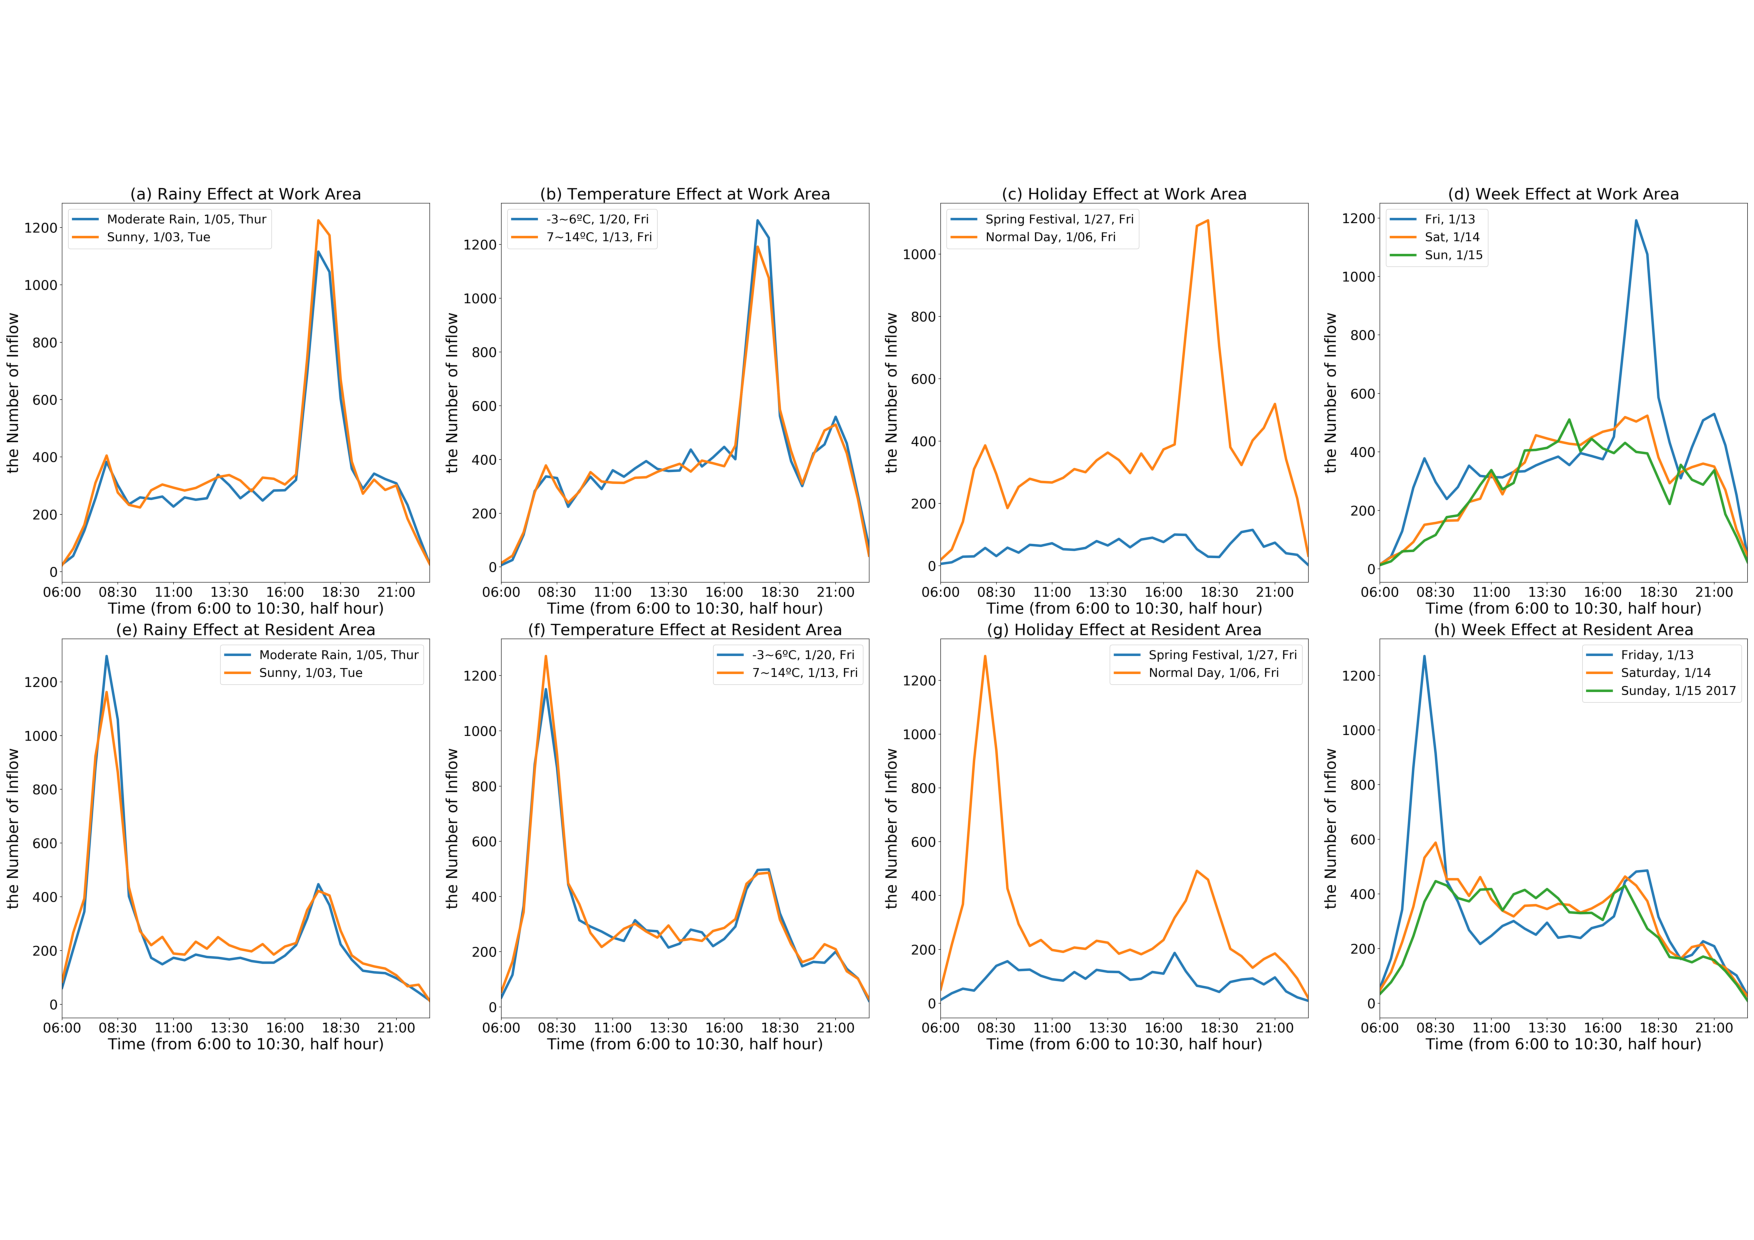
\includegraphics[width=18cm]{external.pdf}}
\caption{Influences of holidays, weather and weekend in Work Area and Resident Area (the area is targeted in Fig.~\ref{fig3}).}
\label{fig6}
\end{figure*}
Traffic flows can be affected by many complex external factors, such as weather and event. Fig.~\ref{fig6} (a) and (e) shows that the effect of moderate rain obviously increase the inflow at the peak time in work and resident area. Fig.~\ref{fig6} (b) and (f) shows that the influence of low temperature increase the crowd inflow at at both area with the  same pattern of moderate rain. Fig.~\ref{fig6} (c) and (g) shows that crowd inflow during Spring Festival can be significantly different from the inflow during normal day at all day time slots. Fig.~\ref{fig6} (d) and (h) shows that Saturday or Sunday has no evidently peak, at resident area morning peak at 8:30pm changing into slow growth for not going to work in morning and at work area as the minority working with no evening peak at 5:30pm. At each comparison, we try to ensure that other factors, showing at each sub figures' legend, are the same.

Let $E_t$ be the extern feature tensor that denotes all external factors at predicted time slot t. In this model (ST-DRN), we primarily concern holiday, weather, and metadata (Workday and Weekends). The details are introduced in Table \uppercase\expandafter{\romannumeral2}. To predict flows at time  t, the holiday and metadata can be straightly obtained by checking the calendar. But the weather at future time slot t is unknown. Usually, one can use the forecasting weather at time slot t or the close weather at time slot $t-1$. Standardly, we employ two fully-connected layers on $E_t$, the first layer is an embedding layer for each sub-factor followed by an activation. The second layer is applied to map low to high dimensions that have the same shape as $X_t$. The output of the external component in Fig.~\ref{fig3} is denoted as $X_{Ex}$ with the parameters $\theta_{Ex}$.

\subsection{Fusion}
At first, we aggregate the first three parts \cite{10} (i.e. nearby, day, week) of Fig.~\ref{fig1} as follows:
\begin{equation}
X_{RU} = W_n \otimes X_n^{\left (L+2 \right )} + W_d \otimes X_d^{\left (L+2 \right )} + W_w \otimes X_w^{\left (L+2 \right )}\label{4}
\end{equation}
where $\otimes$ denotes Hadamard product (i.e., element-wise multiplication), $W_n$, $W_d$ and $W_w$ are the learnable parameters that adjust the degrees influenced by \emph{nearby}, \emph{day} and \emph{week}, respectively.


Then, we here straightly fuse the output of the first three parts with that of the external part, as shown in Fig.~\ref{fig1}. Finally, the predicted value at the $t^{th}$ time slot, denoted by $X_t^\#$, is defined as:
\begin{equation}
X_t^\#=tanh\left (X_{RU} + X_{Ex} \right )\label{5}
=======
where * represents the convolution1; f is an activation function, e.g. the rectifier $f(x) := max(0, x)$ \cite{11}; $W_n^{(1)}$, $b_n^{(1)}$ are the learnable parameters in the first layer. In our ST-DRN (see ''Fig. \ref{fig3}''), we adopt L residual units on Conv1 as follows. On top of the $L^{th}$residual unit, we append a one-dimensional convolutional layer (i.e. Conv2 shown in ''Fig. \ref{fig1}''). With 2 convolutions and L residual units, the output of the nearby part of ''Fig. \ref{fig1}'' is $X_n^{(L+2)}$.

Moreover, As the same procedures mentioned above, we build the day and week parts of ''Fig. \ref{fig1}''. Assume that there are $l_d$ time slots from the day segment and the week is w. Therefore, the day dependent sequence is
$\left [X_{t-l_d.d}, X_{t-(l_d-1).d}, \cdots, X_{t-d}\right ]$. With the convolutional operation and L residual units like in ''\eqref{2}'' and ''\eqref{3}'', the output of the day part is $X_d^{(L+2)}$. Analogously, the output of the week part is $X_w^{(L+2)}$ with the input $\left [X_{t-l_w.w}, X_{t-(l_w-1).w}, \cdots, X_{t-w}\right ]$ where $l_w$ is the length of the week dependent sequence and w is the week span. Note that d and w are actually two different types of periods. Comprehensively, d is equal to one-day that depicts daily periodicity, and w is equal to weekly that draws the one-week tendency.

\subsection{External Elements}
Traffic flows can be affected by many complex external factors, such as weather and event. ''Fig. \ref{fig6}'' (a) and (e) shows that moderate rain obviously increase the inflow at the peak time in work and resident area. ''Fig. \ref{fig6}'' (b) and (f) shows that low temperature increase the crowd inflow at at both area with the  same pattern of moderate rain. ''Fig. \ref{fig6}'' (c) and (g) shows that crowd inflow during Spring Festival can be significantly different from the inflow during normal day at all day time slots. ''Fig. \ref{fig6}'' (d) and (h) shows that Saturday or Sunday has no evidently peak, at resident area morning peak at 8:30pm changing into slow growth for not going to work in morning and at work area as the minority working with no evening peak at 5:30pm. At each comparison, we try to ensure that other factors, showing at each sub figures' legend, are the same.

Let $E_t$ be the extern feature tensor that denotes all external factors at predicted time slot t. In this model (ST-DRN), we primarily concern holiday, weather, and metadata (Workday and Weekends). The details are introduced in Table \uppercase\expandafter{\romannumeral2}. To predict flows at time  t, the holiday and metadata can be straightly obtained by checking the calendar. But the weather at future time slot t is unknown. Usually, one can use the forecasting weather at time slot t or the close weather at time slot $t-1$. Standardly, we employ two fully-connected layers on $E_t$, the first layer is an embedding layer for each sub-factor followed by an activation. The second layer is applied to map low to high dimensions that have the same shape as $X_t$. The output of the external component in ''Fig. \ref{fig3}'' is denoted as $X_{Ex}$ with the parameters $\theta_{Ex}$.

\begin{figure}[htbp]
\small
\centerline{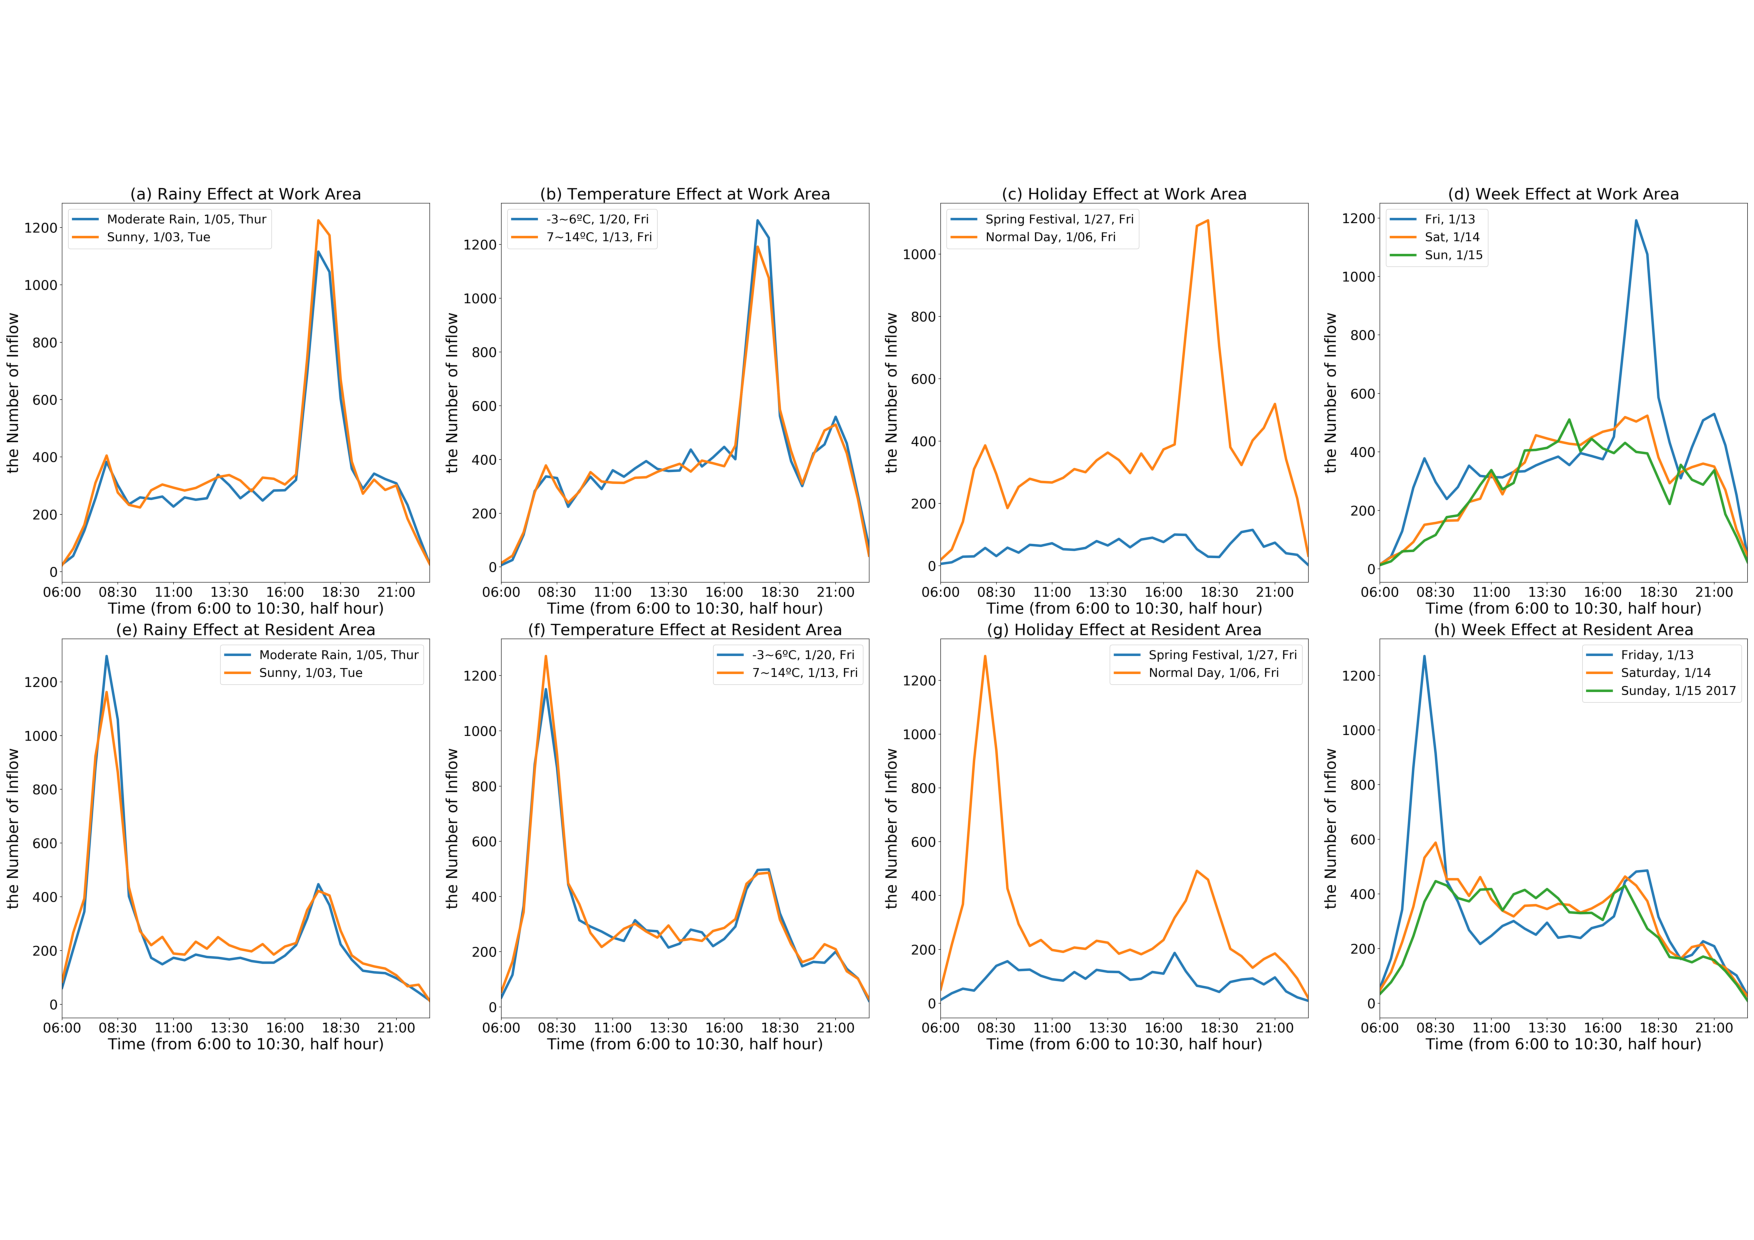
\includegraphics[width=9cm]{external.pdf}}
\caption{Influences of holidays, weather and weekend in Work Area and Resident Area (the area is targeted in ''Fig. \ref{fig3}'').}
\label{fig6}
\end{figure}

\subsection{Fusion}
At first, we aggregate the first three parts \cite{10} (i.e. nearby, day, week) of ''Fig. \ref{fig1}'' as follows:
\begin{equation}
X_{RU} = W_n \otimes X_n^{\left (L+2 \right )} + W_d \otimes X_d^{\left (L+2 \right )} + W_w \otimes X_w^{\left (L+2 \right )}\label{4}
\end{equation}
where $\otimes$ denotes Hadamard product (i.e., element-wise multiplication), $W_n$, $W_d$ and $W_w$ are the learnable parameters that adjust the degrees influenced by nearby, day and week, respectively.

Then, we here straightly fuse the output of the first three parts with that of the external part, as shown in ''Fig. \ref{fig1}''. Finally, the predicted value at the $t^{th}$ time slot, denoted by $\widehat{X}_t$, is defined as:
\begin{equation}
\widehat{X}_t=tanh\left (X_{RU} + X_{Ex} \right )\label{5}
>>>>>>> bd017bd6b8aa7e5822fa100cfe12d52184bfedc4
\end{equation}
where tanh, the activation function, is a hyperbolic tangent that guarantees values of output are at $\left [-1, 1 \right ]$.

Our ST-DRN will be trained to predict $X_t$ from three sequences of flow tensors and external factor features by minimizing mean squared error between the predicted flow
matrix and the true flow matrix:
\begin{equation}
<<<<<<< HEAD
\alpha(\theta) =  \left \|X_t^\# - X_t  \right \|_2^2\label{6}
=======
\alpha(\theta) =  \left \|\widehat{X}_t - X_t  \right \|_2^2\label{6}
>>>>>>> bd017bd6b8aa7e5822fa100cfe12d52184bfedc4
\end{equation}
where �� represents all learnable parameters in the ST-DRN.

\subsection{Algorithm and Optimization}
Algorithm 1 outlines the process of ST-DRN training. We first establish the training instances from the original sequence data. Then, ST-DRN is trained by back-propagation (BP) and Adam \cite{4}.
\begin{algorithm}[ht]
\caption{ST-DRN Training Algorithm}

\begin{algorithmic}

\renewcommand{\algorithmicrequire}{\textbf{Input:}}
\renewcommand{\algorithmicensure}{\textbf{Output:}}

\REQUIRE
    \STATE Lengths of nearby, day, week sequences: $l_n, l_d, l_w$;
    \STATE Day period: $d$; week period: $w$;
    \STATE External factors: $\left \{E_0, \dots, E_{n-1} \right \}$;
    \STATE Historical data: $\left \{X_0, \dots, X_{n-1} \right \}$;

\ENSURE
    \STATE Learned ST-DRN model
\end{algorithmic}
~
\begin{algorithmic}[1]
\STATE $//$ step1: establish training instances
\STATE $M \gets \phi$

\FORALL {$all\ time\ slots\ t\ (1\le t \le (n-1))$}
\STATE $D_n=\left [X_{t-l_n}, X_{t-\left (l_n-1 \right )}, \dots, X_{t-1} \right ]$
\STATE $D_d=\left [X_{t-l_d.d}, X_{t-\left (l_d-1 \right ).d}, \dots, X_{t-d} \right ]$

\STATE $D_w=\left [X_{t-l_w.w}, X_{t-\left (l_w-1 \right ).w}, \dots, X_{t-w} \right ]$

// $X_t$ is the target at time slot t
<<<<<<< HEAD

\STATE place an training instance $(\left \{D_n, D_d, D_w, E_t \right \}, X_t)$ into $M$
\ENDFOR
~
=======
\STATE place an training instance $(\left \{D_n, D_d, D_w, E_t \right \}, X_t)$ into $M$
\ENDFOR

~\\
>>>>>>> bd017bd6b8aa7e5822fa100cfe12d52184bfedc4
\STATE $//$step2: training model
\STATE Init all learnable parameters $\theta$ in ST-DRN

\REPEAT
\STATE randomly select a batch of instances $M_t$ from $M$
<<<<<<< HEAD
\STATE find $\theta$ by minimizing the formula in \eqref{6} with $M_t$
=======
\STATE find $\theta$ by minimizing the formula in ''\eqref{6}'' with $M_t$
>>>>>>> bd017bd6b8aa7e5822fa100cfe12d52184bfedc4
\UNTIL $stopping\ criteria\ is\ met$

\end{algorithmic}
\end{algorithm}


\section{Evaluation}
We use the record data collected from subway AFC system of Suzhou in time span from 1st September. 2016 to 31th January. 2017. And we process this data into inflow and outflow 30 minutes as a time slot from 6:00 to  22:30 for each station at every day. Then we use the last month's data to test ST-DRN model and the remaining to train this model. Again, we use this way to train and test our baseline models. We use the ARIMA and SARIMA model to compare ST-DRN.
<<<<<<< HEAD
\subsection{Baselines}
\textbf{ARIMA:} Auto-Regressive Integrated Moving Average (ARIMA) \cite{16} is a well-known model for understanding and predicting future values, one of the popular linear models in time series forecasting during the past three decades (reference). Although ARIMA models are extremely, representing several different types of time series, i.e., autoregressive (AR), moving average (MA) and combined AR and MA (ARMA) series. P, Q, D are 3, 34, 2 respectively representing the order of AR, MA and Difference.

\textbf{SARIMA:} Seasonal ARIMA \cite{15}. A seasonal ARIMA model is formed by including additional seasonal terms in the ARIMA models we have seen so far. Seasonality in a time series is a regular pattern of changes that repeats over a regular time periods. S is 3 representing the order of seasonal character adding from ARIMA model.

\textbf{ANN:} It first extracts the temporal features in each station, and feed into an artificial neural network \cite{17}, applying just to pattern the relationship between past and current to forecast the future flows with the same hyper parameters installed in ST-DRN.

\subsection{Preprocessing}
We use tanh as our final activation in the output of the ST-DRN in Fig.~\ref{fig1}, whose range is between -1 and 1. Hence, we transform the flows data into the range $[-1, 1]$ by the Min-Max normalization method. In the evaluation, we shift the predicted value back to the normal values, compared with the truth flows data. For external factors, we transform weekends or workday, holidays and weather conditions into binary tensors by one-hot code, and use Min-Max normalization to map the Temperature and Wind speed into the range $\left [0, 1 \right ]$.

\subsection{Hyper parameters}
=======

\subsection{Baselines}
\textbf{ARIMA:} Auto-Regressive Integrated Moving Average (ARIMA) \cite{16} is a well-known model for understanding and predicting future values, one of the popular linear models in time series forecasting during the past three decades (reference). Although ARIMA models are extremely, representing several different types of time series, i.e., autoregressive (AR), moving average (MA) and combined AR and MA (ARMA) series.

\textbf{SARIMA:} Seasonal ARIMA \cite{15}.

\textbf{ANN:} It first extracts the temporal features in each station, and fed into an artificial neural network \cite{17}, applying just to pattern the relationship between past and current to forecast the future flows.

\subsection{Preprocessing}
We use tanh as our final activation in the output of the ST-DRN in ''Fig. \ref{fig1}'', whose range is between -1 and 1. Hence, we transform the flows data into the range $[-1, 1]$ by the Min-Max normalization method. In the evaluation, we shift the predicted value back to the normal values, compared with the truth flows data. For external factors, we transform weekends or workday, holidays and weather conditions into binary tensors by one-hot code, and use Min-Max normalization to map the Temperature and Wind speed into the range $\left [0, 1 \right ]$.

\subsection{Parameters}
>>>>>>> bd017bd6b8aa7e5822fa100cfe12d52184bfedc4
The python libraries, including Keras and Theano, are used to build our models. The convolutions of Conv1 and all residual units use 64 filters of size $59\times1$ (one-dimensional), and Conv2 uses a convolution with 2 filters of size $59\times1$. The batch size and learning rate are 32, 0.0001 respectively. We partition 80\% of the training data for training model, and the remaining is chosen as the validation set, which is used to early-stop our training algorithm for each model based on the best validation score. Afterwards, we continue to train the model on the full training data for a fixed number of epochs (e.g., 150 epochs). There are 5 extra parameters in our model, of which p and q are empirically fixed to the number of time slots at one-day and one-week, respectively. For choices of the three dependent sequences, we propose them as: $l_n\in\mathnormal{\left \{3, 4, 5 \right \}}$, $l_d\in\mathnormal{\left \{1, 2, 3, 4 \right \}}$, $l_w\in\mathnormal{ \left \{1, 2, 3, 4 \right \}}$.

\begin{table}[htbp]
\caption{Data sets (AFC record data , holidays, weekends and weather conditions)}
\begin{center}
\begin{tabular}{|c|c|c|c|}
\hline
\multicolumn{2}{|c|}{\textbf{Data set}}&\multicolumn{2}{|c|}{\textbf{Subway}} \\
\hline
\multicolumn{2}{|c|}{Data type} & \multicolumn{2}{|c|}{Subway AFC record data} \\
\multicolumn{2}{|c|}{Location} & \multicolumn{2}{|c|}{Suzhou} \\
\multicolumn{2}{|c|}{Time span} & \multicolumn{2}{|c|}{ From 9/1 2016 to 1/31 2017} \\
\multicolumn{2}{|c|}{Length of time slot} & \multicolumn{2}{|c|}{ 30 minutes} \\
\multicolumn{2}{|c|}{The number of stations} & \multicolumn{2}{|c|}{ 59} \\
\hline
\multicolumn{4}{|c|}{\textbf{Statistic information of flows for each station}}\\
\multicolumn{4}{|c|}{\textbf{at a time slot on January 2017}} \\
\hline
Inflow & max: 2536 & mean: 136 & std: 167.906 \\
Outflow & max: 3113 & mean: 137 & std: 170.365 \\
\hline
\multicolumn{4}{|c|}{\textbf{Statistic information of external data}}\\
\hline
\multicolumn{2}{|c|}{Holidays} & \multicolumn{2}{|c|}{ 13 days} \\
\multicolumn{2}{|c|}{Weekends} & \multicolumn{2}{|c|}{ 44 days} \\
<<<<<<< HEAD
\multicolumn{2}{|c|}{The number of weather} & \multicolumn{2}{|c|}{ 5 types (e.g. Sunny, Rainy)} \\
=======
\multicolumn{2}{|c|}{The number of stations} & \multicolumn{2}{|c|}{ 7 types (e.g. Sunny, Rainy)} \\
>>>>>>> bd017bd6b8aa7e5822fa100cfe12d52184bfedc4
\multicolumn{2}{|c|}{Temperature ($C^\circ$)} & \multicolumn{2}{|c|}{ $\left [-3, 34 \right ]$} \\
\hline
\end{tabular}
\label{tab2}
\end{center}
\end{table}

Evaluation Metric: We measure our method by Root Mean Square Error (RMSE) as:
\begin{equation}
<<<<<<< HEAD
RMSE = \sqrt{\frac{1}{a}\cdot \sum_{ i}^{ }(X_i-X_i^\#)^2 }\label{7}
\end{equation}
where $x^\#$ and $x$ are the predicted value and truth data, respectively; a denotes the number of all predicted values.


\subsection{Results on AFC Data}
As shown in Fig.~\ref{fig7}, We first give the comparison with baseline models on Suzhou. We provide several variants of ST-DRN with different layers and different factors. Taking L4 for example, it defaulted contains external factors, 40 length of one-dimensional convolution kernel, and has 4 residual units, each of which is consisted of two convolutional layers and before ReLU with batch normalization (BN) as Fig.~\ref{fig2}. As default, the three dependent sequences are $\left \{3, 1, 1 \right \}$ with the order of $l_n$, $l_d$, $l_w$. Comparing with the previous baseline models and the different types of ST-DRN, L4 reduces error to 27.809, which perfectly improves accuracy. ST-DRN has relatively from 34.29\% up to 58.16\% lower RMSE than three baselines, demonstrating that our proposed model has good performance on flow prediction tasks. However, L4+A1 or L4+A2, using early an hour data before predicted time t, has approximative RMSE with these baselines, demonstrating that our model has not perfectly performance on Non real-time system and inspiring us to modify the model in future. Respectively, the RMSE values of ANN, ARIMA and SARIMA are 55.401, 66.473, 63.130.
\begin{itemize}
\item \textbf{Number of residual unit:} Results of L2, L4 show that RMSE decreases as the number of residual units increases. On theory, the effects of result increase with adding residual unit layer and we need more data to feed the deeper network, using residual learning. However L6 show poor effect than L4, as the learning rate and batch size same in two experiment or the limited data. Respectively, the RMSE values of L2 and L6 are 31.529, 34.461.
\item \textbf{Distinct structure of residual unit:} We try some different types of residual units. L4 adopts the standard Residual Unit without special note (see Fig.~\ref{fig2}). Compared with L4, Residual Unit of L4+SingleRU only contains 1 ReLU followed by 1 convolution and 1 BN before ReLU, and Residual Unit of L4+NoBN remove two batch normalization layers, each of which is placed before ReLU. We observe that L4+NoBN is worse than L4, and L4+NoBN is better than L4+SingleRU, demonstrating the effectiveness of batch normalization and more convolution, respectively. Separately, the RMSE values of L4+SingleRU and L4+NoBN are 33.079, 31.123.
\item \textbf{External elements:} L4 considers the external factors, including weekends, holiday and weather. If not, the model is denoted as L4+NoE. The results, that L4 is better than L4+NoE, reveal that external factors are always advantageous.
\item \textbf{Parametric matrix fusion:} Being different with L4, L4+NoFusion do not use parametric matrix fusion (see Eq. 4). Instead, L4+NoFusion use a straightforward method for fusing, i.e., $X_n^{(L+2)} + X_d^{(L+2)} + X_w^{(L+2)}$. It shows the error greatly increases, which evidences the effectiveness of our used parametric matrix fusion. Respectively, the RMSE values of L4+NoE and L4+NoFusion are 32.751, 30.219.
\item \textbf{size of convolution kernel:} As we thoroughly discuss in subsection Spatio Components in section \uppercase\expandafter{\romannumeral3}, the different size of convolution kernel has different effect on this data and the best size is around 40, decided by the layout of metro stations, the distribution of ride time length, and the metro stations numbering sequence. Respectively, the RMSE values of L4+10, L4+35 and L4+50 are 36.407, 30.795, 33.963.
\item \textbf{Early data:} Mentioned at Introduction, we adjust the parameters for ST-DRN to attempt using early one hour data. L4+A1 using $\left \{l_n, l_d, l_w \right \}$ of $\left \{1, 3, 1\right \}$ show better performs than L4+A2 setting $\left \{l_n, l_d, l_w \right \}$ of $\left \{3, 1, 1\right \}$ and baseline models in Table \uppercase\expandafter{\romannumeral3}. And the results reveal our model's practical value and guide us to modify ST-DRN at actually using in subway system in the future. Respectively, the RMSE values of L4+A1 and L4+A2 are 58.964, 63.692.
\end{itemize}

\begin{figure}[htbp]
\small
\centerline{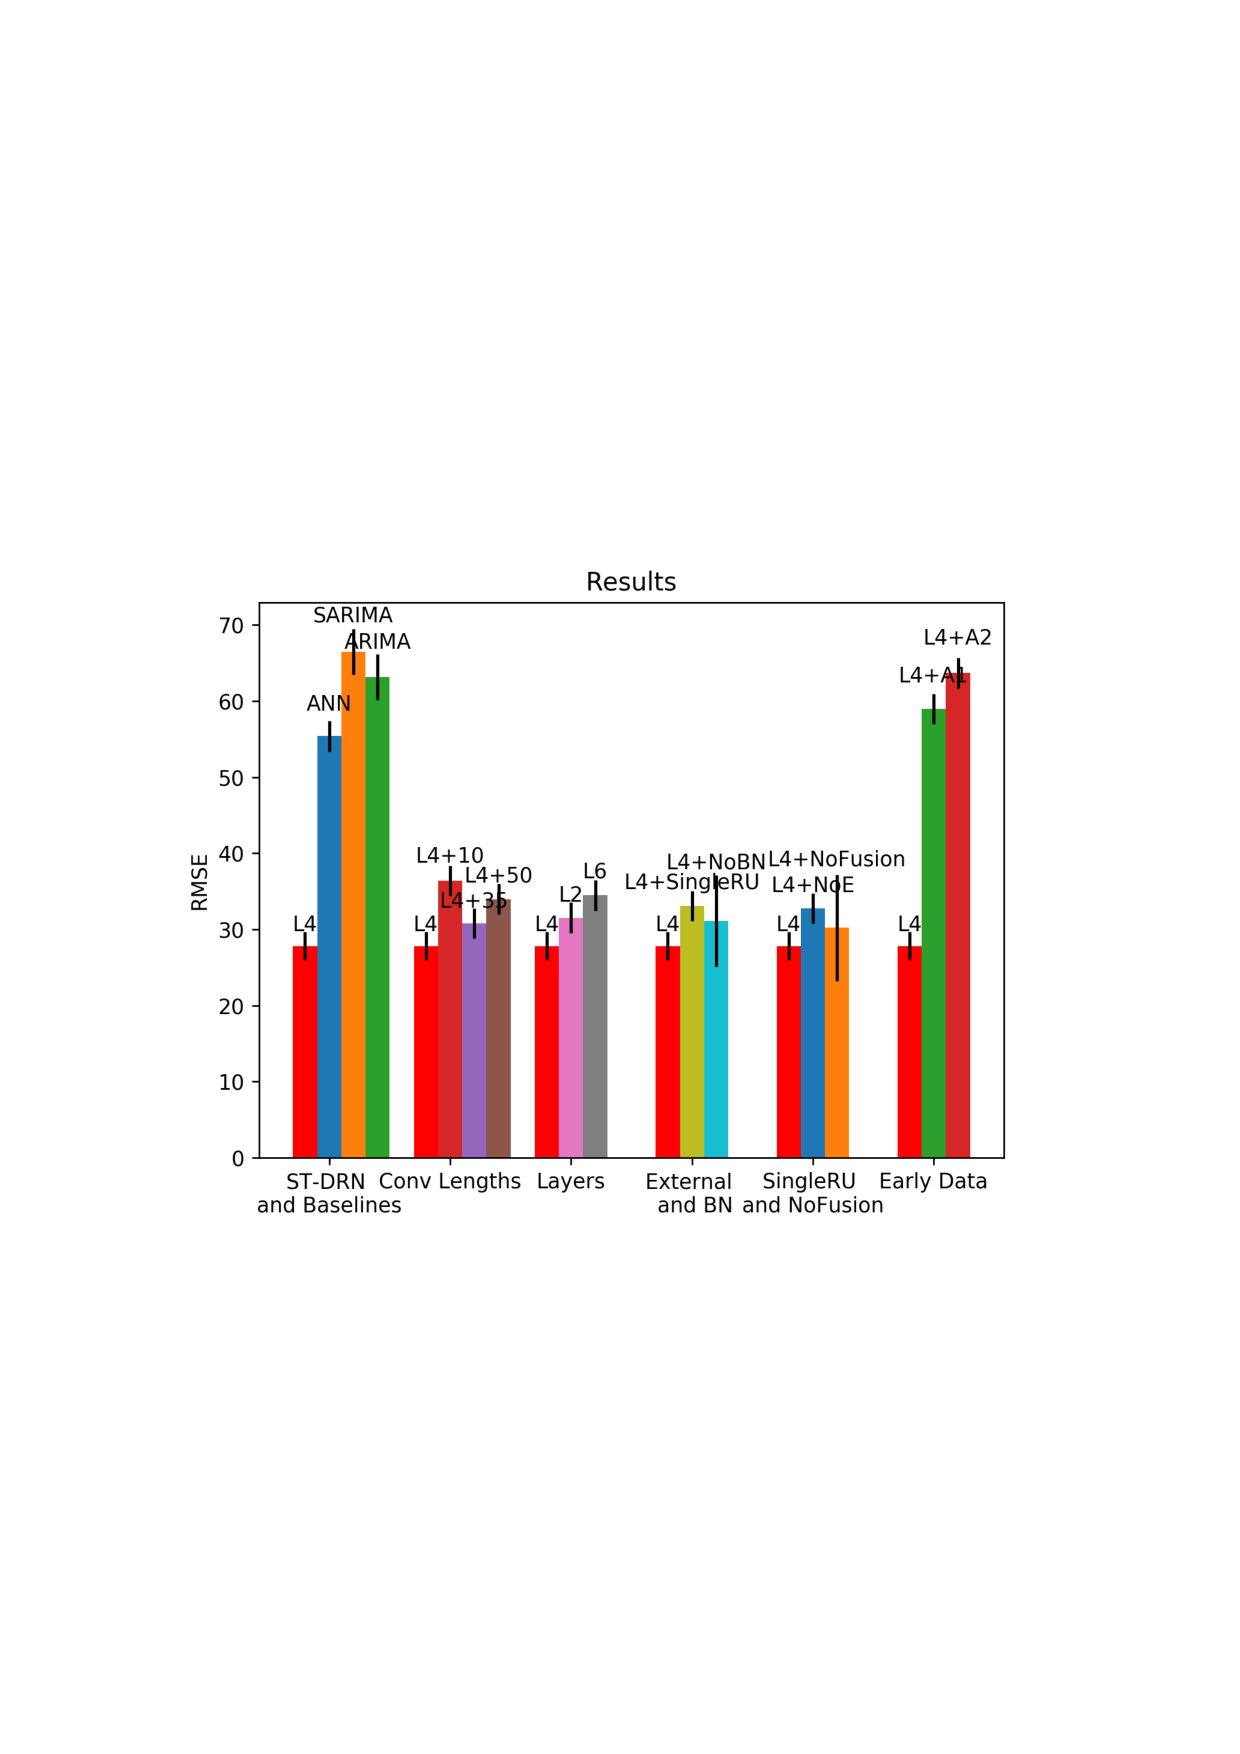
\includegraphics[width=9cm]{results.pdf}}
\caption{Results on AFC Data}
\label{fig7}
\end{figure}

\subsection{Discussions}
In above results, we find that L4, the best forecasting model we proposed, is promoted than ARIMA \cite{16} by 55.94\% and L4+A1 is little better than AIMAR in accuracy. Hence, our model make a great improvement in forecasting accuracy with fast training model time using GPU, as the layer of deep residual network is light, if AFC data can be real time collected by system.


\section{Conclusion}
In this paper, to pattern particular spatio-temporal forecast validly \cite{20}, we mainly propose applying the residual learning, inserting CNNs in residual unit in Fig.~\ref{fig2} to handle spatial issue, and a parametric matrix fusion mechanism to integrate the three sub-factors of temporal. We use deep residual learning model for forecasting the flow of crowds in each subway station, based on historical data, weather, weekends and holidays. We evaluate our model on two types of crowd flows in Suzhou AFC record data, attaining significantly performances than 3 baseline methods, making sure that our model is better and more applicable to the flow prediction on subway station.
=======
RMSE = \sqrt{\frac{1}{a}\cdot \sum_{ i}^{ }(X_i-\widehat X_i)^2 }\label{7}
\end{equation}
where $\widehat{x}$ and x are the predicted value and truth data, respectively; a denotes the number of all predicted values.


\subsection{Results on AFC data}
As shown in Table \uppercase\expandafter{\romannumeral3}, We first give the comparison with baseline models on Suzhou. We provide several variants of ST-DRN with different layers and different factors. Taking L4+40+E for example, it considers external factors, 40 meaning the length of  one-dimensional convolution kernel, and has 4 residual units, each of which is consisted of two convolutional layers and before ReLU with batch normalization (BN) as ''Fig. \ref{fig2}''. As default, the three dependent sequences are $\left \{3, 1, 1 \right \}$ with the order of $l_n$, $l_d$, $l_w$. Comparing with the previous baseline models and the different types of ST-DRN, L4+40+E reduces error to 29.809, which perfectly improves accuracy. And L4+40+E+A1 or L4+40+E+A2, using early an hour data before predicted time t, has some effects than baseline models.

\begin{itemize}
\item \textbf{Number of residual unit:} Results of L2+40+E, L4+40+E show that RMSE decreases as the number of residual units increases. On theory, the effects of result increase with adding residual unit layer and we need more data to feed the deeper network, using residual learning. However L6+40+E show poor effect than L4+40+E, as the learning rate and batch size same in two experiment.
\item \textbf{Distinct structure of residual unit:} We try some different types of residual units. L4+40+E adopts the standard Residual Unit without special note (see ''Fig. \ref{fig2}''). Compared with L4+40+E, Residual Unit of L4+40+E+single-RU only contains 1 ReLU followed by 1 convolution and 1 BN before ReLU, and Residual Unit of L2+40+E+No-BN remove two batch normalization layers, each of which is placed before ReLU. We observe that L2+40+E+No-BN is worse than L2+40+E, and L4+40+E is better than L4+40+E-single-RU, demonstrating the effectiveness of batch normalization and more convolution, respectively.
\item \textbf{External elements:} L4+40+E considers the external factors, including weekends, holiday and weather. If not, the model is denoted as L4+40. The results, that L4+40+E is better than L4+40, reveal that external factors are always advantageous.
\item \textbf{Parametric matrix fusion:} Being different with L4+40+E, L4+40+E+No-Fusion do not use parametric matrix fusion (see Eq. 4). Instead, L4+40+E+No-Fusion use a straightforward method for fusing, i.e., $X_n^{(L+2)} + X_d^{(L+2)} + X_w^{(L+2)}$. It shows the error greatly increases, which evidences the effectiveness of our proposed parametric matrix fusion.
\item \textbf{size of convolution kernel:} As we thoroughly discuss in subsection Spatio Components in section \uppercase\expandafter{\romannumeral3}, the different size of convolution kernel has different effect on this data and the best size is around 40, decided by the layout of metro stations, the distribution of ride time length, and the metro stations numbering sequence.
\item \textbf{Early data:} Mentioned at Introduction, we adjust the parameters for ST-DRN to attempt using early one hour data. L4+40+E+A1 using $\left \{l_n, l_d, l_w \right \}$ of $\left \{1, 3, 1\right \}$ show better performs than L4+40+E+A2 setting $\left \{l_n, l_d, l_w \right \}$ of $\left \{3, 1, 1\right \}$ and baseline models in Table \uppercase\expandafter{\romannumeral3}. And the results reveal our model's practical value and guide us to modify ST-DRN at actually using in subway system in the future.
\end{itemize}

\begin{table}[htbp]
\caption{Comparison different modles on Suzhou AFC.}
\begin{center}
\begin{tabular}{|c|c|c|c|}
\hline
\multicolumn{3}{|c|}{\textbf{Baseline model}} & \multicolumn{1}{|c|}{\textbf{RMSE}} \\
\hline
\multicolumn{3}{|c|}{ARIMA} & \multicolumn{1}{|c|}{ 75.130} \\
\multicolumn{3}{|c|}{SARIMA} & \multicolumn{1}{|c|}{ 78.473} \\
\multicolumn{3}{|c|}{ANN} & \multicolumn{1}{|c|}{ 67.401} \\
\hline
\multicolumn{3}{|c|}{\textbf{ST-DRN}} & \multicolumn{1}{|c|}{\textbf{RMSE}}\\
\hline
\multicolumn{3}{|c|}{ L2+40+E} &\multicolumn{1}{|c|}{33.529}\\
\multicolumn{3}{|c|}{ L2+40+E+No-BN} &\multicolumn{1}{|c|}{36.843}\\
\hline
\multicolumn{3}{|c|}{ L4+40} &\multicolumn{1}{|c|}{34.751}\\
\hline
\multicolumn{3}{|c|}{ L4+40+E+single-RU} &\multicolumn{1}{|c|}{33.079}\\
\hline
\multicolumn{3}{|c|}{ L4+40+E+No-Fusion} &\multicolumn{1}{|c|}{32.219}\\
\hline
\multicolumn{3}{|c|}{ L4+40+E} &\multicolumn{1}{|c|}{29.809}\\
\multicolumn{3}{|c|}{ L4+35+E} &\multicolumn{1}{|c|}{32.795}\\
\multicolumn{3}{|c|}{ L4+10+E} &\multicolumn{1}{|c|}{38.402}\\
\multicolumn{3}{|c|}{ L4+50+E} &\multicolumn{1}{|c|}{35.963}\\
\hline
\multicolumn{3}{|c|}{ L6+40+E} &\multicolumn{1}{|c|}{36.461}\\
\hline
\multicolumn{3}{|c|}{ L4+40+E+A1} &\multicolumn{1}{|c|}{58.964}\\
\multicolumn{3}{|c|}{ L4+40+E+A2} &\multicolumn{1}{|c|}{63.692}\\
\hline
\end{tabular}
\label{tab3}
\end{center}
\end{table}

\subsection{Algorithm iteration process}
\begin{figure}[htbp]
\small
\centerline{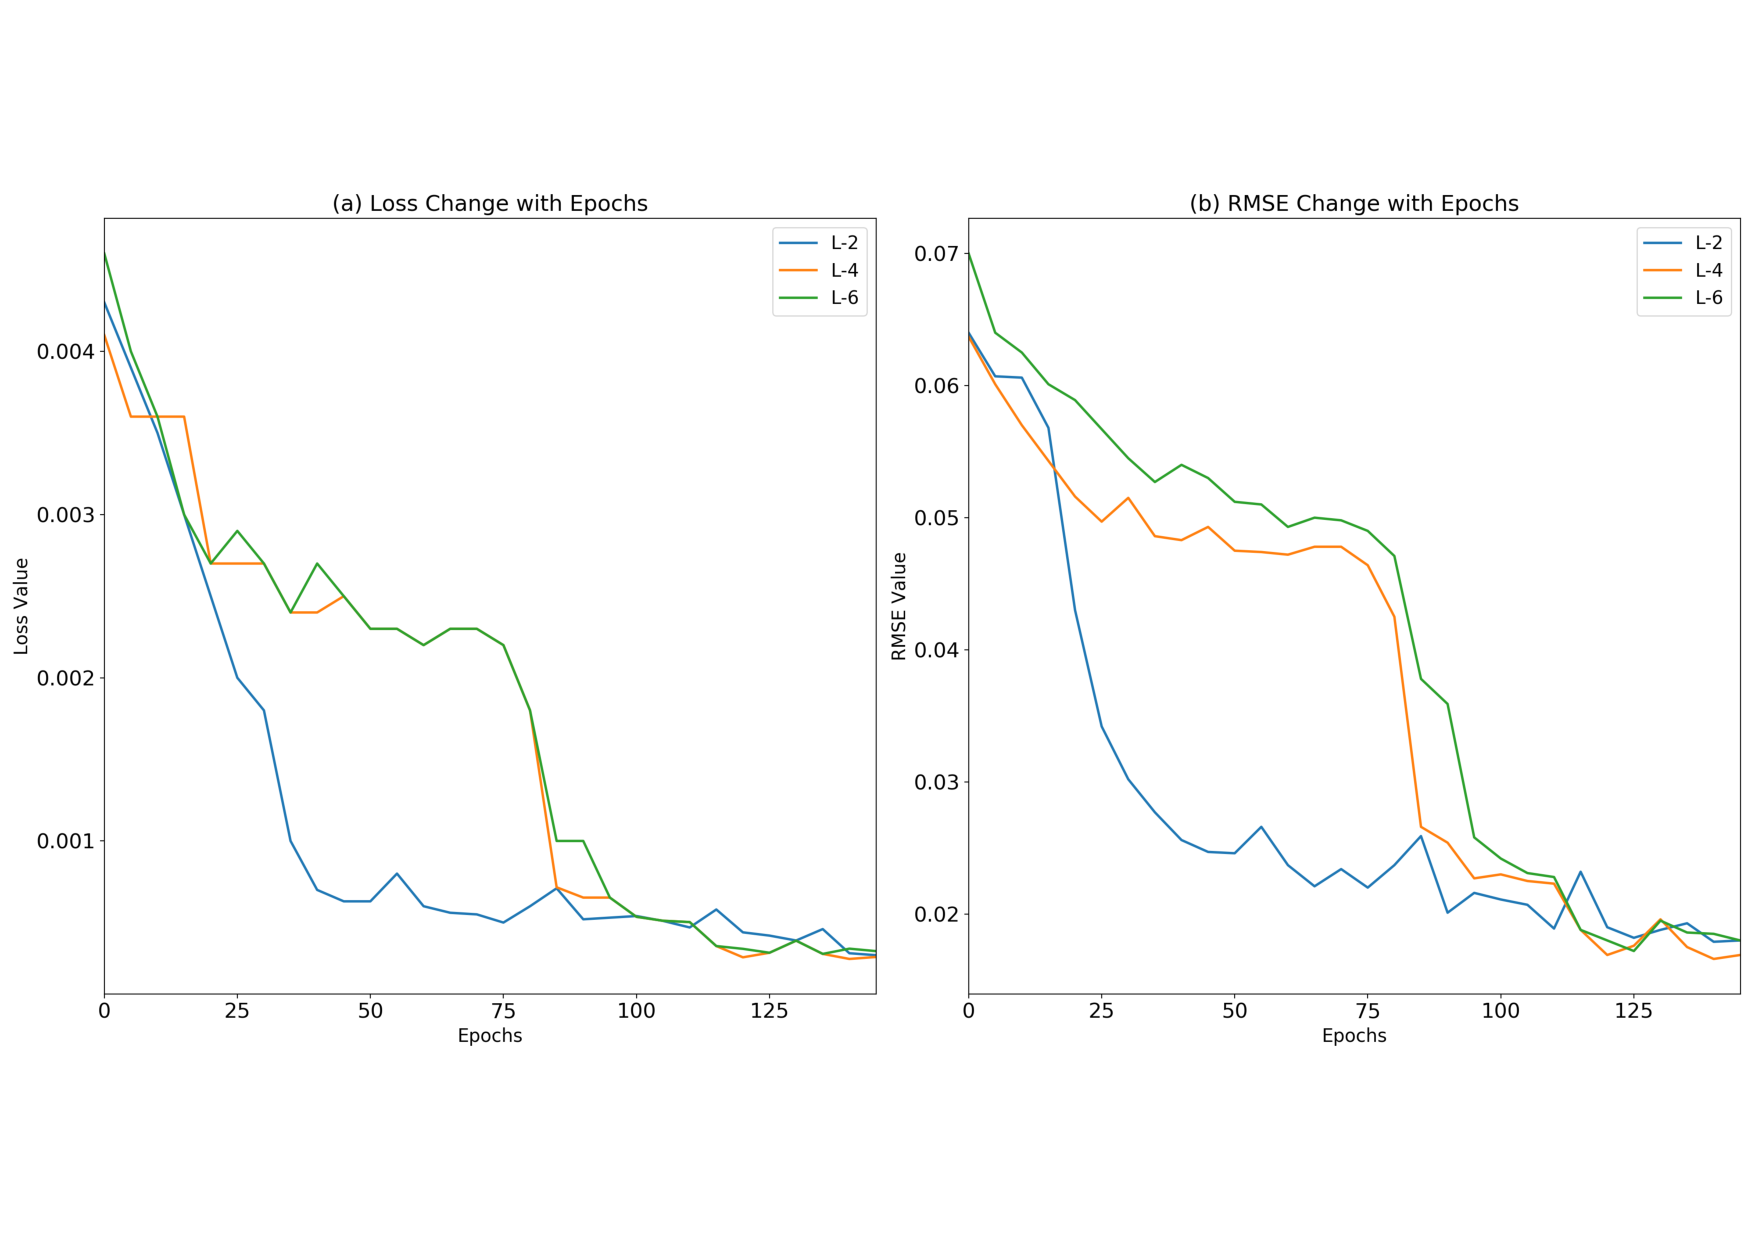
\includegraphics[width=9cm]{rmse.pdf}}
\caption{Iteration process}
\label{fig7}
\end{figure}
We use the data generated in  L2+40+E, L6+40+E and L6+40+E iteration process to draw ''Fig. \ref{fig7}''. Intuitively, it reveal our model the process of train,  L4 having most the same procession with L6 and lately convergence than L2. But L4 has the best performance than L2 and L4, so with this data set our model showing best is with 4 layers residual units.


\section{Conclusion and Future Work}
There are some previously published works on predicting flows in metro based on historical passenger data collected in the automatic fare collection (AFC) system to improve on advertising efficiency at subway system \cite{14} and also to reduce last-mile distances from metro station to destination and decrease travel time using cellphones, vehicles and smartcard data \cite{21}. They predict millions or billions of individuals�� mobility traces rather than the aggregated crowd flows in an area. Some other researchers predict travel traffic flow on the road by joint probability distribution between the cause nodes (data utilized for forecasting) and the effect node (data to be forecasted) in a constructed Bayesian network \cite{7}. Most of them are predicting single or multiple road segments, rather than citywide ones. These work are not considering the dependencies among areas and using history data not effectively and comprehensively than us.

CNNs have been universally applied to various problems, especially displaying unparalleled effect in the field of computer vision \cite{11}. Residual learning allows such networks to have a very super deep structure \cite{1} and recurrent neural networks (RNNs) \cite{8} have been generally employed for sequence learning tasks \cite{12}. However, both kinds of neural networks can only capture spatial or temporal dependencies.

In this paper, to pattern particular spatio-temporal forecast validly \cite{20}, we mainly propose applying the residual learning, inserting CNNs in residual unit in ''Fig. \ref{fig2}'' to handle spatial issue, and a parametric matrix fusion mechanism to integrate the three sub-factors of temporal. We use deep residual learning model for forecasting the flow of crowds in each subway station, based on historical data, weather, weekends and holidays. We evaluate our model on two types of crowd flows in Suzhou AFC record data, attaining significantly performances than 3 baseline methods, making sure that our model is better and more applicable to the flow prediction on subway station.

In the future, we consider using two ways to upgrade our model and be applicable in reality. On the one hand, we will discern the type of passengers, having regular riding trace \cite{18} such as between office and home at workdays and apply the irregular data in this model to train. On the other hand, we can adjust the temporal parameters to improve the performance on early data.
>>>>>>> bd017bd6b8aa7e5822fa100cfe12d52184bfedc4

\bibliographystyle{IEEEtran}
\bibliography{my}


\end{document}
